\documentclass[review]{elsarticle}
\usepackage{amsmath,amssymb,amsfonts}
\usepackage{array}
\usepackage{booktabs}
\usepackage{changepage}
\usepackage{rotating}  %used for "sidewaystable" // gsc 2010.11.14
\usepackage{txfonts}
\usepackage[linesnumbered,ruled]{algorithm2e}
%\usepackage{cite}
\usepackage{amssymb}
\usepackage{rotating}
\usepackage{setspace}
%\usepackage{algorithm}
%\usepackage{algorithmic}
%\usepackage[ruled,vlined]{algorithm2e}
\usepackage{graphicx}
\usepackage{subcaption}
\usepackage{amsmath}
\usepackage{multirow}
\usepackage{epstopdf}
\usepackage{color}
\usepackage{float}
\usepackage{appendix}
\newtheorem{remark}{Remark}
\usepackage{yhmath}
\usepackage[table]{xcolor}
\definecolor{modColor}{rgb}{0,0,1}
%opening

\begin{document}
	\begin{frontmatter}
	\title{Reinforcement Learning-based Particle Swarm Optimization for Wind Farm Layout Problems}
	\author[label1]{Zihang Zhang} %zhangzhstu@gmail.com
	\author[label1]{Jiayi Li}%lijiayi212@gmail.com
	\author[label1]{Zhenyu Lei} %
	\author[label1]{Qianyu Zhu} %Syukennu@gmail.com
	\author[label2]{Jiujun Cheng}%chengjj@tongji.edu.cn
	\author[label1]{Shangce Gao\corref{cor1}}\ead{gaosc@eng.u-toyama.ac.jp}
	\address[label1]{Faculty of Engineering, University of Toyama, Toyama-shi, 930-8555 Japan.}
	\address[label2]{Key Laboratory of Embedded System and Service Computing, Ministry of Education, Tongji University, Shanghai, 200092 China.}
		\cortext[cor1]{Corresponding author}
\begin{abstract}

\textcolor{blue}{Optimizing wind farm layouts is critical to maximizing wind power generation. The wake effect significantly impacts turbines located downwind, making farm layout a key determinant of power generation efficiency. Traditional algorithms often overlook the value of leveraging historical information, which can lead to entrapment in local optima. Our survey reveals that previous studies on wind farm layout optimization (WFLO) have not adequately integrated the historical data of particle swarm optimization (PSO) with reinforcement learning’s empirical pool, resulting in the loss of valuable information. Here, we present a novel approach that enhances algorithm development and exploration by utilizing historical data and integrating proximal policy optimization from reinforcement learning with an experience pool. This method markedly outperforms the conventional genetic PSO in terms of performance. Extensive numerical experiments across wind farms of various sizes and four distinct wind scenarios demonstrate the superior efficacy of our reinforcement learning-based particle swarm optimization (RPSO) algorithm compared to 12 state-of-the-art methods. Under four wind scenarios, the average power conversion efficiencies of RPSO for the three turbine scales reach 98.68$\%$, 98.14$\%$, and 97.33$\%$, respectively, underscoring the high competitiveness of the proposed RPSO for WFLO in diverse wind conditions.}

\end{abstract}

\begin{keyword}
wind farm layout optimization \sep proximal policy optimization \sep particle swarm optimizer  \sep wake effect
\end{keyword}

\end{frontmatter}

\section{Introduction}
To address the global warming crisis, the development and utilization of renewable energy are imperative. Among these, wind energy stands out as a pivotal alternative to fossil fuels due to its affordability, widespread availability, and environmental sustainability \cite{cheng2014state, mohammadi2013using, kadri2020energy}. In 2022, global wind power generation witnessed a remarkable increase of 17$\%$, solidifying its position as a key energy source for the future as recognized by an expanding array of nations.

The efficiency of wind turbine power generation hinges on various factors. Previous studies have predominantly focused on maximizing power generation efficiency through wind speed prediction, optimization of wind turbine models, modeling wake effects, and optimizing wind turbine layouts. The downstream wake effect phenomenon significantly curtails the output power of downstream turbines due to interference from upstream turbines. Optimizing turbine layout offers a viable strategy to mitigate the impact of wake effects and thereby maximize array power generation efficiency, rendering it a pivotal area of investigation. Despite the widespread adoption of advanced intelligent algorithms for layout optimization, traditional approaches still grapple with suboptimal solutions, susceptibility to local optima, and instability \cite{zhang2020dynamic, zhang2021soft, zhao2020review, jang2022techno}.

To address these challenges, this work proposes a Genetic Particle Swarm Optimization (PSO) based on Proximal Policy Optimization (PPO) reinforcement learning (RL) algorithm \cite{cai2020provably, kuznetsova2013reinforcement}. PPO is a new type of Policy Gradient algorithm. Traditional Policy Gradient algorithms rely heavily on the selection of the step size, but it is also difficult to determine the appropriate step size, which leads to too large a difference between the old and new policies during training, and is not conducive to learning \cite{gu2021proximal}. PPO solves the problem of step size selection by realizing small batch updating in multiple training steps. In the Genetic PSO algorithm, $r$ is a parameter which controls the proportion of the current optimal individual in the next generation of heredity. The selection of optimal particles and the genetic ratio can greatly affect the efficiency of the PSO algorithm, and in previous studies, this ratio $r$ is chosen randomly and sum to 1, or at a constant value from past studies, which may not be an appropriate approach for different problems \cite{zhang2022proximal}. Therefore, we introduce the PPO algorithm to utilize the empirical pool data to help the PSO algorithm determine $a$ better $r$ for higher power generation efficiency.

This work compares the proposed algorithm with other state-of-the-art (SOTA) algorithms applied to wind turbine layout optimization under the same experimental conditions. The experimental results show that the proposed algorithm outperforms the other algorithms for three sizes of wind farms (30, 35, and 40 turbines), four wind scenarios. Also, the proposed algorithm is competitive in the ablation experiments, which demonstrate the significant improvement of RL on the original algorithm.

The main highlights and contributions of this work can be summarized as follows:

\begin{itemize}
	\item [1)] In this work, the proposed method of combining RL with traditional intelligent algorithms is applied to wind turbine layout optimization. Extensive numerical experiments show that the proposed method outperforms all the twelve SOTA models compared in this problem.
	\item [2)] RL utilizes historical search information to break out of otherwise constrained conditions and help guide the PSO to converge in a better direction.
	\item [3)] Instead of the previous approach of random selection in PSO, we employ the PPO strategy. Furthermore, we introduce two independent parameters to replace the original constraint of their summation equalling 1. Experimental results unequivocally demonstrate that this novel methodology significantly enhances solution quality.
\end{itemize}

The rest of the paper is structured as follows: Section \ref{relatedwork} summarizes the work related to wind turbines. Section \ref{wflonm} presents the numerical model for the wind turbine layout optimization problem. Section \ref{prorpso} describes the proposed algorithm in detail. Experimental results are presented in Section \ref{experimental}. Section \ref{conclusion} summarizes the work in this paper.

\section{Related work}\label{relatedwork}

To maximize wind turbine output efficiency, researchers typically examine various factors including wind farm siting, wind speed prediction, wind turbine design, wake flow modeling, and wind farm layout optimization (WFLO). As energy technology continues to advance, optimization of wind turbine design and wake modeling has become increasingly efficient and stable. Consequently, WFLO has emerged as a crucial aspect in enhancing the power generation capacity of wind farms \cite{rezaeiha2020framework, chen2020medium}. WFLO involves optimizing the positioning of each wind turbine within the array to minimize wake effects between turbines and maximize overall power generation capacity. As the number of turbines increases, optimizing wake effects becomes increasingly challenging \cite{saad2020performance}.

In the past, extensive efforts have been dedicated to improving WFLO through the optimization of intelligent algorithms. Generally, WFLO problems can be approached through two main methods: discrete modeling and continuous modeling. Discrete modeling involves placing wind turbines at the centers of pre-defined grids of equal size. The finer the division of the wind field, the more intricate the WFLO problem that can be addressed. Conversely, continuous modeling permits turbines to be placed anywhere within the grid, not necessarily at the center. However, this approach typically entails higher computational complexity and is highly sensitive to initialization. In \cite{mosetti1994optimization}, Mosetti et al. used genetic algorithms (GA) for the first time in the Jensen wake model to solve the discrete WFLO problem. They divide the wind farm into equal-sized grids of a certain size, and each grid is used to place a turbine. Subsequently, Marmidis et al. \cite{marmidis2008optimal} further divided the wind farm gridding, subdivided into 100 squares with higher accuracy, and solved the WFLO by Monte Carlo simulation. \textcolor{blue}{Cheng et al. \cite{cheng2022design} used three optimization algorithms, GA, PSO and simulated annealing, and a back-propagation neural network-based machine learning approach to optimize a novel U-type Darrieus Wind Turbine (UDWT). The results show that the UDWT can improve aerodynamic and structural performance compared with conventional two- and four-blade wind turbines. Recently, Neshat et al. \cite{neshat2024enhancing} proposed a novel, robust and efficient multi-objective swarm optimisation approach (DMOGWA) to achieve an optimal compromise between maximising the power output of a wave energy converter and minimising the impact on the nacelle acceleration of a wind turbine. This approach is applied to hybrid offshore renewable energy platforms to optimise power production and reduce the levelised cost of energy by integrating or sharing several renewable energy technologies. Experimental results show that DMOGWA has advantages over many well-known multi-objective swarm intelligence methods and mainstream evolutionary multi-objective algorithms.} In GA, Grady et al. \cite{grady2005placement} improved the GA algorithm by proposing a method to improve the number of individual iteration steps to optimize the discrete WFLO problem. In \cite{emami2010new}, Emami and Noghreh propose a new objective function that better balances the cost, power, and efficiency of wind farms, and then encode the GA algorithm in a new way, so that the algorithm no longer relies on subpopulations, and can be solved with a single genetic algorithm. Chen et al. \cite{chen2013wind} used a nested genetic algorithm to optimize the layout of wind turbines with different hub heights and further demonstrated the effectiveness of the proposed approach on a large commercial wind farm. In 2015, Chen et al. \cite{chen2013wind} further used a multi-objective genetic-based algorithm to optimize wind farm layout, again experimenting under real commercial wind farms. Ju et al. \cite{ju2019wind} proposed Adaptive Genetic Algorithm (AGA) and Self-Inspired Genetic Algorithm (SIGA) to address the limitations of traditional GA. The worst turbines were randomly relocated using AGA, and then SIGA was used to re-direct the localization. Subsequently, Ju et al. \cite{ju2019winda} proposed a support vector regression-based bootstrap genetic algorithm to optimize the layout of wind farms by considering landowner participation. For the first time, Wang et al. \cite{wang2017differential} proposed a differential evolution algorithm with a new coding mechanism by treating the position of each turbine as an individual. The whole population then represents a layout, reducing the dimension of the search space and eliminating the population size parameter. Yu et al. \cite{yu2023chaotic} proposed a differential evolutionary family of algorithms with chaotic local search-based as well as enhanced memory storage mechanisms for WFLO.

Not limited to EAs, other types of intelligent algorithms have also demonstrated efficacy in addressing the WFLO problem. Feng et al. \cite{feng2015solving} introduced an enhanced randomized search (RS) algorithm employing a continuous formulation. Experimental results highlighted the algorithm's performance, which was attributed to both GAs and previous RS algorithms. In \cite{erouglu2012design}, the authors presented an enhanced ACO algorithm tailored for the WFLO problem, specifically addressing wake effects. Their work yielded notable progress in this domain. \textcolor{blue}{Bai et al. \cite{bai2022wind} further improved the utilisation of the adaptive genetic algorithm proposed by the previous authors by transforming the relocation of multiple wind turbines into a single-player reinforcement learning problem, which was further solved by Monte Carlo tree search embedded in an evolutionary algorithm. Experimental results show that the proposed method brings significant improvements over previous methods.} Hou et al. \cite{hou2015optimized} employed the PSO algorithm to optimize a mathematical model they proposed, which incorporates variations in wind direction and wake losses. Their objective was to maximize energy output while minimizing total production costs. Pookpunt and Ongsakul \cite{pookpunt2013optimal} introduced a binary PSO method with time-varying acceleration coefficients. They demonstrated the effectiveness of their approach in addressing the WFLO problem through experimental comparisons with numerous variants. Tao et al. \cite{tao2019optimal} utilized a hybrid Gray Wolf Optimization algorithm to address the WFLO problem, integrating multiple wind turbine placement strategies. They achieved promising results, particularly when employing the Frandsen-Gaussian wake model. An adaptive genetic learning particle swarm optimization method for optimizing the WFLO problem was proposed by Lei et al \cite{lei2022adaptive}. The strategy adaptively adjusts the position of the worst turbine to improve the conversion efficiency of the wind farm. Later, the same authors improved the PSO algorithm by a chaotic local search mechanism for optimizing large-scale WFLO problems with good results \cite{lei2023chaotic}.

In recent years, more and more researchers have tried to use RL to optimize various single-objective and multi-objective problems. Dong and Zhao \cite{dong2023reinforcement} propose an automatic grouping method for wind turbines based on RL, and their proposed automatic grouping strategy enables large-scale wind farms to be divided into subgroups that are favorable for RL training. Bai et al. \cite{bai2022wind} leveraged an adaptive genetic algorithm, integrating Monte Carlo Tree Search to iteratively relocate wind turbine layouts to more optimal positions, resulting in notable performance improvements. Yu and Lu \cite{yu2023reinforcement} introduced a Q-Learning based multi-objective differential evolutionary algorithm to address the WFLO problem. By utilizing Q-Learning, the authors fine-tuned the parameters of the differential evolution algorithm, achieving a balance between local and global searches. Yu and Zhang \cite{yu2023teaching} introduced a teaching optimization algorithm based on RL. Through adjustments to the structure of the original algorithm, performance was optimized. The enhanced algorithm surpassed other algorithms in performance across two simulated wind conditions and four wind farm scenarios. In \cite{dong2021intelligent}, the authors demonstrated a significant improvement in power generation for wind farms by utilizing sparse datasets through a novel deep RL-based wind farm control scheme. Remarkably, this approach does not necessitate wake-up modeling. In \cite{xie2021wind}, the authors employed deep RL to optimize the thrust coefficient and yaw angle, leading to a significant enhancement in the total power generation of a wind farm.

\section{Wind farm layout numerical model}\label{wflonm}
In this section, we begin by introducing the most crucial wake model utilized in wind farm optimization. Subsequently, we outline the objective function and evaluation methods employed in this study.

\begin{table}[htbp]
	\captionsetup{labelfont={color=black},font={color=black}}
	\centering
	\scriptsize
	\caption{The nomenclature used in this article.}
	\resizebox{0.7\columnwidth}{!}{
		\begin{tabular}{l l}\hline
			Symbol&Description \\\hline
			{$\pi$}&{The ratio of the circumference}\\
			{$r$}&{The diameter of rotors}\\
			{$R$}&{The radius of influence of wake effect}\\
			{$v$}&{The number of velocity}\\
			{$h$}&{The height of wind turbine towers}\\
			{$S$}&{The intersecting area of wake effect}\\
			{$d$}&{The distance between two turbines}\\
			{$N$}&{The number of turbines}\\
			{$\Phi$}&{The layout}\\
			{$\eta$}&{The conversion efficiency}\\
			{$\sigma$}&{The wind scenario}\\
			{$p_{i}$}&{The location of turbines}\\
			{$M$}&{The population size}\\
			{$L_{s}$}&{The length of the rows and columns}\\
			{$L_{w}$}&{The width of each grid}\\
			{$D$}&{The dimensions of WFLO}\\
			{$pbest$}&{Individual historical best position}\\
			{$gbest$}&{Particle global optimal position}\\
			{$\pi_{\theta}$}&{The policy of PPO}\\
			{$\epsilon$}&{The hyperparameter for control strategy updating}\\
			{$\mu$}&{The entrainment constant}\\\hline
	\end{tabular}}
	\label{Nomenclature}
\end{table}

\subsection{Wake model}
In a wind farm, the presence of a wind turbine upwind significantly impacts the performance of turbines located downwind, a phenomenon known as the wake effect, illustrated in Fig. \ref{fig:jm}. To mitigate the adverse effects of wake turbulence on overall energy extraction, it is imperative to devise a more optimized layout to enhance energy capture efficiency. In our study, we adopt the Jensen model to assess wind speeds affected by wake, as it is a widely used semi-empirical wake model in engineering. Specifically, wind turbines 1 and 2 are positioned upwind, while wind turbine 3 is situated downwind. As a result of the wake effect, the wind speed experienced by wind turbine 3 is significantly diminished.
\begin{figure}
	\centering
	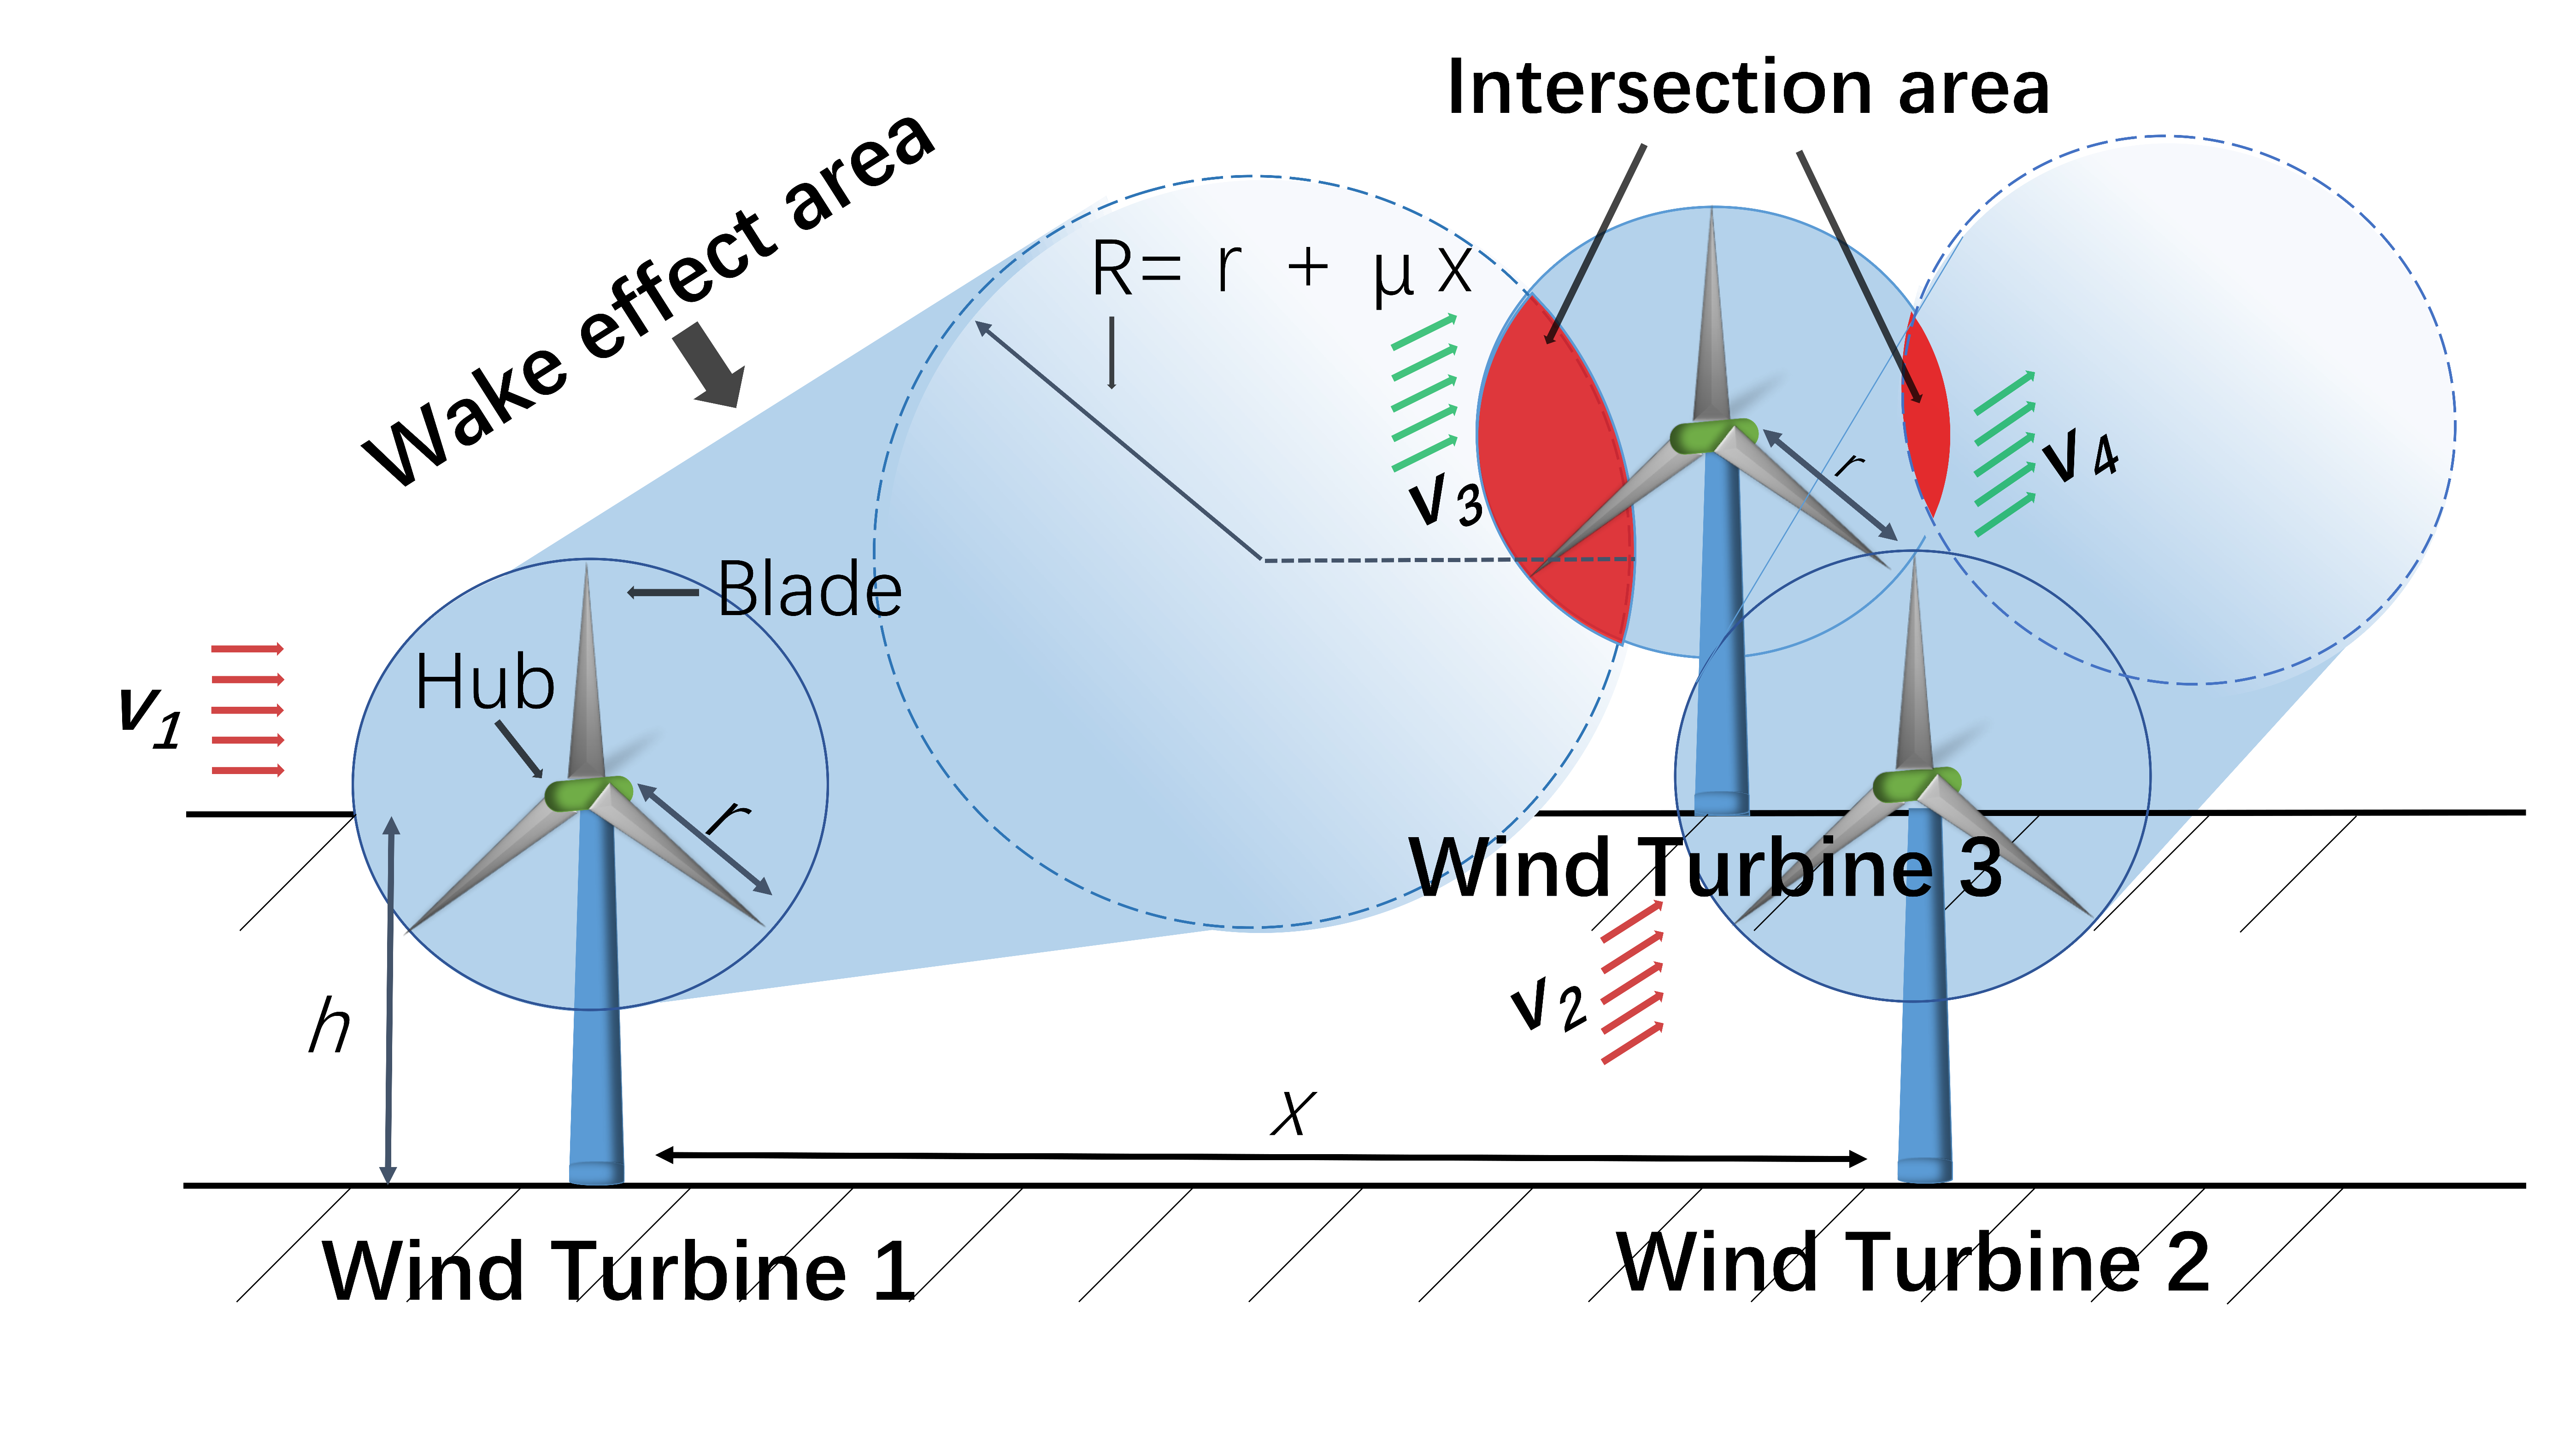
\includegraphics[width=1.0\columnwidth]{JensenModel.eps}
	\caption{The illustration of wake effect.}
	\label{fig:jm}
\end{figure}
\subsubsection{Jensen single wake model}
The Jensen model operates under the assumption of momentum conservation, whereby the momentum deficit undergoes linear variation. Wind turbines separated by $x$ can be expressed as:
\begin{equation}
	\label{mc}
	\pi r^{2}v_{1}^{\prime}+\pi (R^{2}-r^{2})v_{1}=\pi R^{2}v_{3},
\end{equation}

\begin{equation}
	\label{mcdl}
	R=r+\mu x,
\end{equation}
$\mu$ is the entrainment constant:
\begin{equation}
	\label{alp}
	\alpha=\frac{0.5}{ln(\frac{h}{k_{0}})},
\end{equation}
where $k_{0}$ is the roughness of wind farm ground surface, $h$ is the height of wind turbine towers. Meanwhile, this model gives the wind velocity just passing through the turbine $v_{1}^{\prime}$ as approximately equal to $\frac{1}{3}v_{1}$ ambient wind velocity according to classical theory. The downwind turbine velocity $v_{3}$, which is effect of a single wind turbine, can be expressed as \cite{archer2018review}:
\begin{equation}
	\label{3}
	v_{3}=v_{1}\left[1-\frac{2}{3}\left(\frac{r}{r+\frac{0.5}{ln(\frac{h}{k_{0}})} x}\right)^{2}\right].
\end{equation}

\subsubsection{Jensen multiple wake model}
In practical wind farm applications, a wind turbine is influenced by the wake effects generated by multiple upwind turbines, as depicted in Fig. \ref{fig:jm}. Consequently, a single wake effect model is inadequate. Instead, the Jensen multiple wake effect model is employed, with the formula expressed as follows \cite{archer2018review}:
\begin{equation}
	\label{3}
	v=v_{1}\left[1-\sqrt{\sum_{i}^{N}\left(1-\frac{v_{i}}{v_{1}}\right)^{2}
	\left(\frac{S_{i}}{S_{r}}\right)^{2}}\right],
\end{equation}
where $v$ is the combined wind speed of the turbine after it has been subjected to multiple wake effects, $v_{i}$ is the wind speed affected by the wake effect of the $i$-th upwind fan. Note that here we assume that all wind turbines are subjected to an initial velocity ($v_{1}$, $v_{2}$, etc.) that is equal and equal to the ambient wind speed.
\begin{figure}
	\centering
	
\includegraphics[width=1.0\columnwidth]{IntersectedArea.eps}
	\caption{The intersecting area of two turbines.}
	\label{fig:ia}
\end{figure}
$S_{i}$ is the area where the wake effect of the $i$-th turbine intersects the turbine at the downwind location. $S_{r}$ is the surface area of each turbine (assuming that all turbines in the wind farm have the same configuration). The intersecting areas of the two turbines can be roughly divided into the two scenarios of Fig. \ref{fig:ia}.

In all cases, the intersecting area $S_{i}$ is equal:
\begin{equation}
	\label{ia}
	S_{i}=S_{\wideparen{ABD}}+S_{\wideparen{CBD}}-2S_{\triangle{ABC}},
\end{equation}
by the cosine theorem:
\begin{align}
	\label{rad}
	\alpha&=\arccos\left(\frac{R^{2}+d^{2}-r^{2}}{2Rd}\right)\\
	\beta&=\arccos\left(\frac{r^{2}+d^{2}-R^{2}}{2Rd}\right),
\end{align}
substituting radians into the sector formula,
\begin{equation}
	\begin{split}
	\label{ss}
	S_{i}=&\left[\arccos\left(\frac{R^{2}+d^{2}-r^{2}}{2Rd}\right)+\arccos\left(\frac{r^{2}+d^{2}-R^{2}}{2Rd}\right)\right]\cdot R^{2}-Rd\sin(\alpha).
	\end{split}
\end{equation}

Note that the above equation omits the conversion between radian and angle.

\subsection{Objective function of WFLO}
The goal of WFLO is to maximize the overall output of the wind farm while minimizing the adverse effects of wake turbulence on turbine performance, all while minimizing construction costs. The objective function can be expressed as:
\begin{equation}
	\label{objec}
	O=\min\frac{C(N)}{T(N,\sigma,\Phi)},
\end{equation}
where $N$ is the number of turbines in the wind farm. In this study, $N$ is a constant, $T$ is the energy output of the wind field of N turbines under $\sigma$ wind conditions, $\Phi$ layout. $\sigma$ is wind scenario that includes wind speed and direction, etc. $\Phi$ is the wind farm layout. The construction cost uses the formula given in \cite{mosetti1994optimization}:
\begin{equation}
	\label{cn}
	C(N)=N\left(\frac{2}{3}+\frac{1}{3}e^{-0.00174N^{2}}\right).
\end{equation}

Therefore, the objective function can be written to maximize the output of the wind farm \cite{mosetti1994optimization}:
\begin{equation}
	\begin{split}
	\label{max}
	O=&\max T(N,\sigma,\Phi)\\
	=&\sum_{i=1}^{N}\sum_{v,\theta}^{}p(v,\theta)T_{i}(v,\theta,\Phi),
	\end{split}
\end{equation}
where $v$ and $\theta$ are wind speed and wind direction under wind scenario $\sigma$ respectively. $p(v,\theta)$ is the probability of $v$ and $\theta$. In WFLO, it is common to use the conversion efficiency $\eta$ to represent the performance performance of the whole wind farm. Therefore, we use the following equation to represent the performance of the current layout $\Phi$:
\begin{equation}
	\label{eta}
	\eta=\frac{T(N,\sigma,\Phi)}{N\sum\limits_{v,\theta}^{}p(v,\theta)T_{r}(v,\theta,\Phi)},
\end{equation}
where $T_{r}(v,\theta,\Phi)$ is the power rating at wind speed $v$, wind condition $\theta$ and layout $\Phi$. $\eta$ is closer to 1, indicating that the layout is more effective.

\section{Proposed RPSO}\label{prorpso}
\begin{figure*}
	\centering
	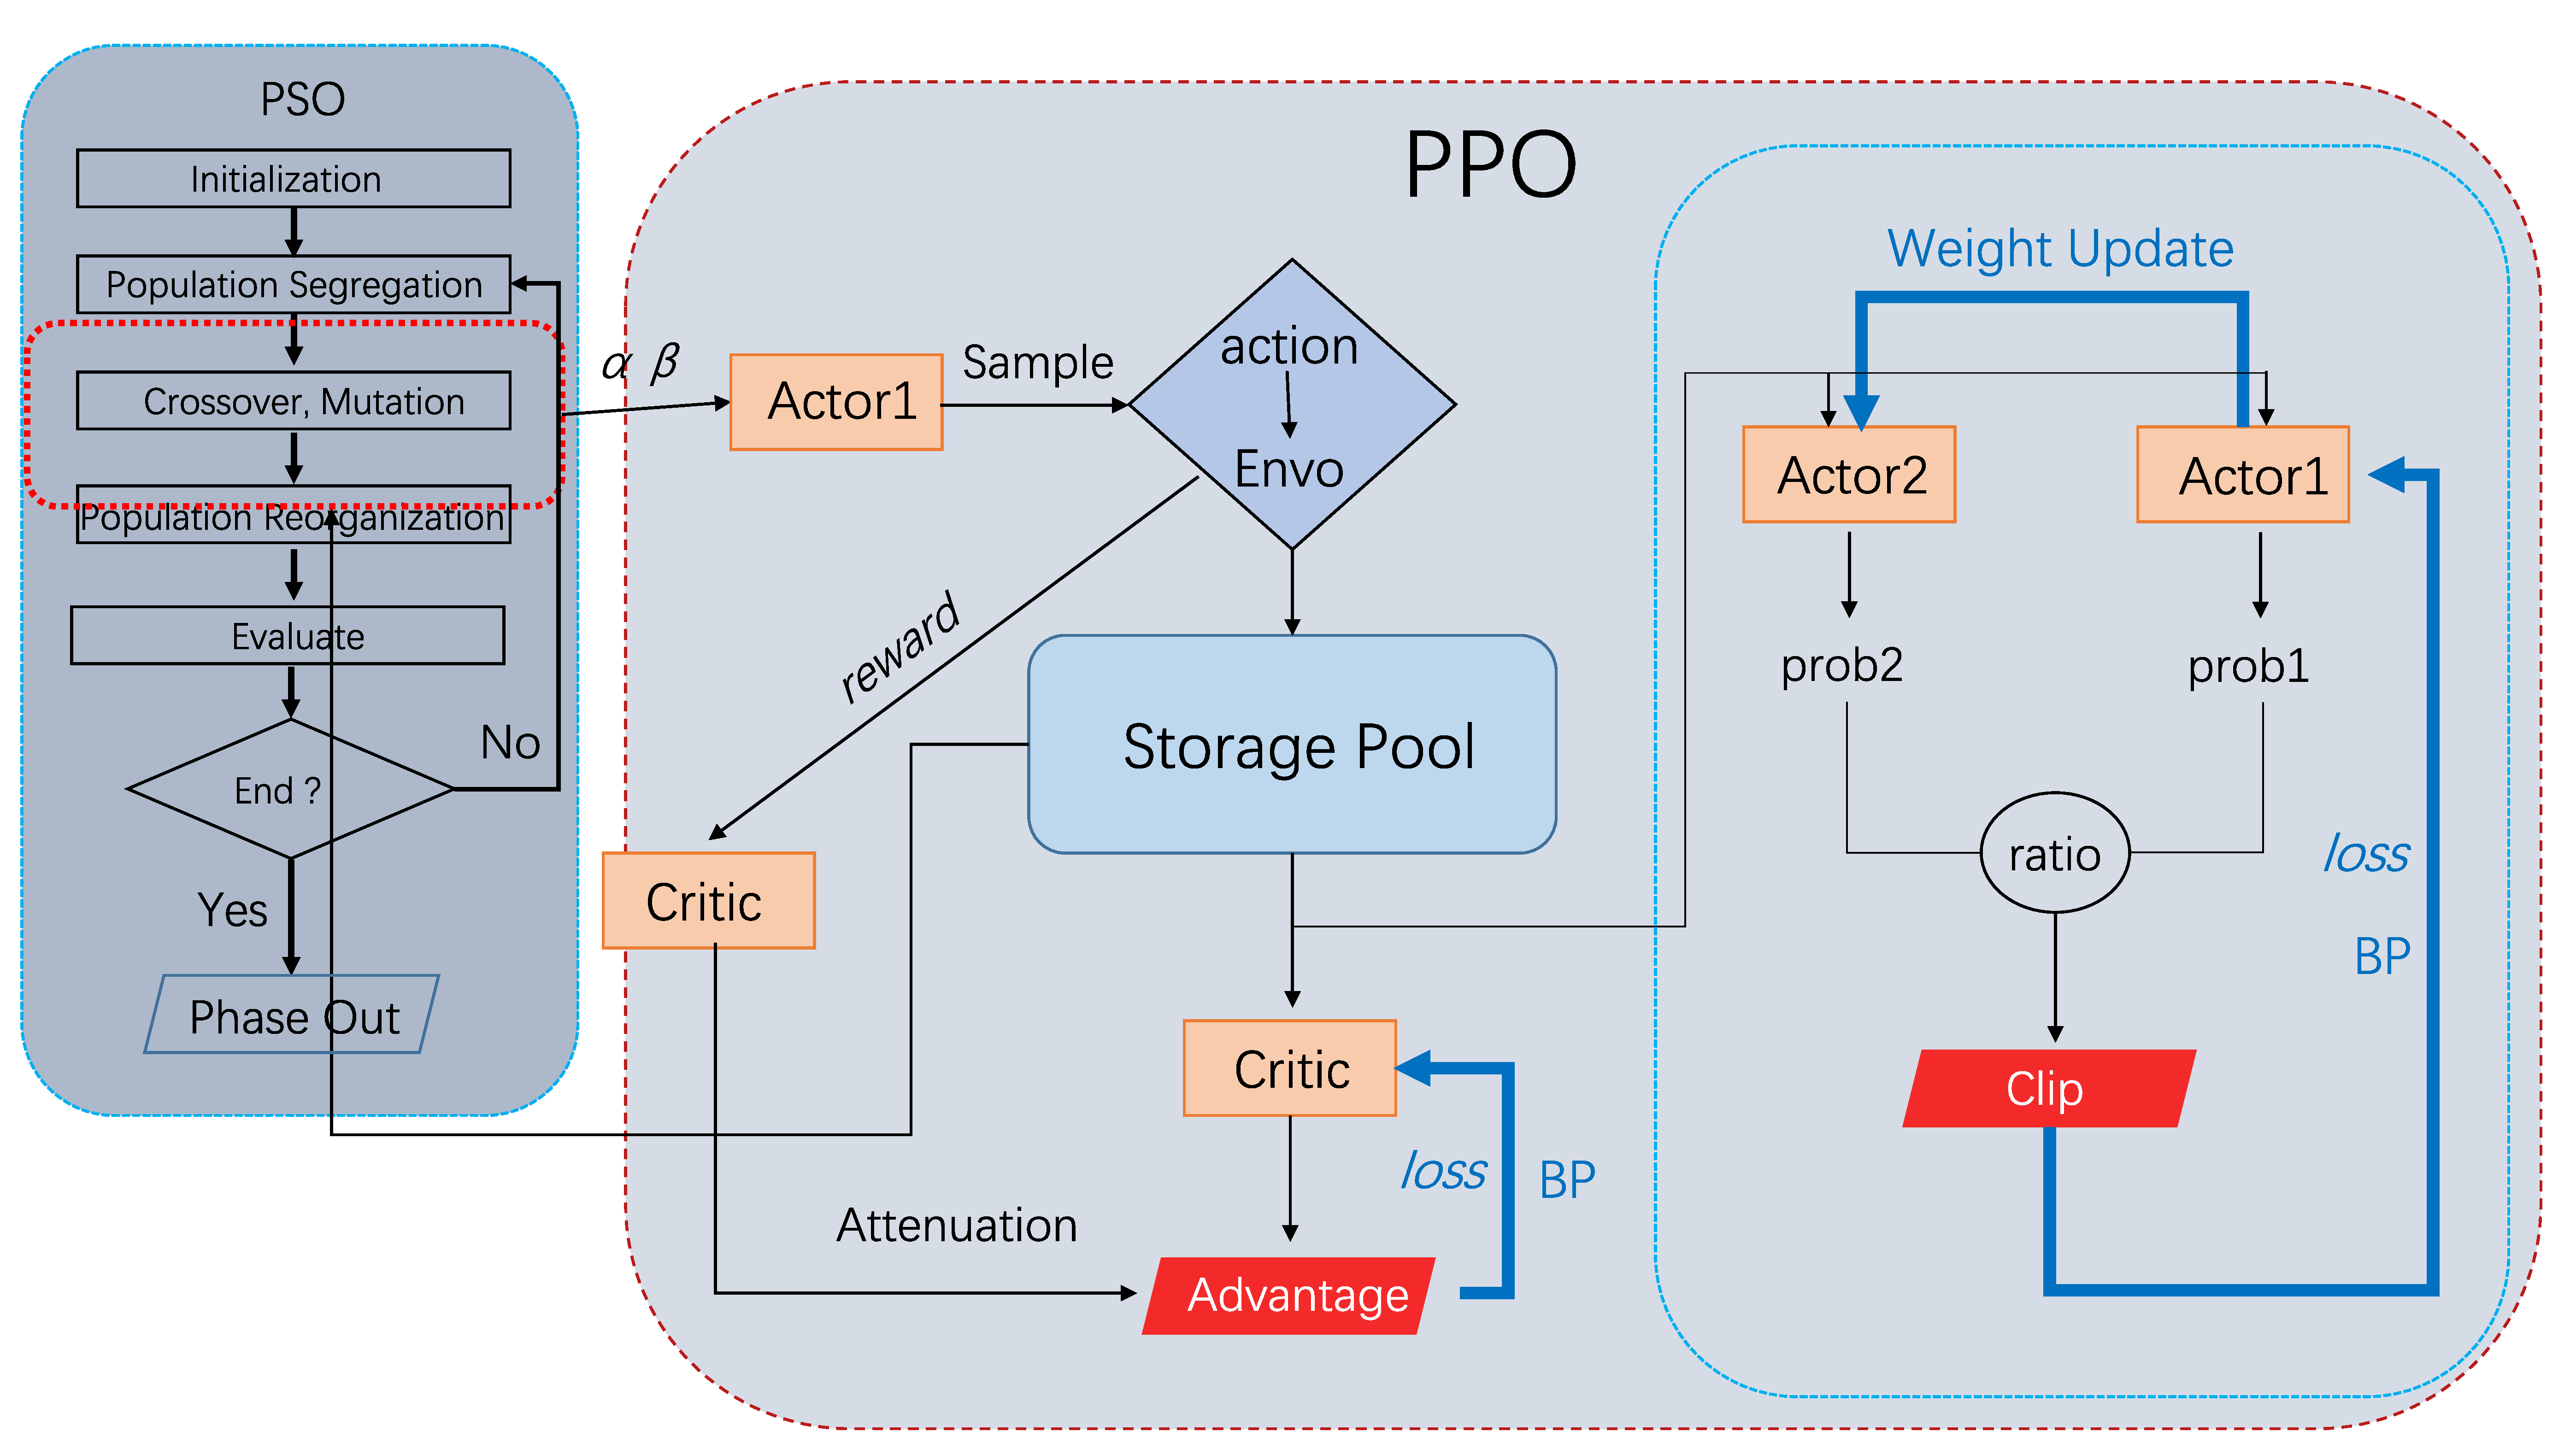
\includegraphics[width=1\textwidth]{rpso.eps}
	\caption{The flowchart of RPSO.}
	\label{flowchart}
\end{figure*}
The proposed reinforcement learning-based particle swarm optimization (RPSO) algorithm is presented in this section. The overall flow of RPSO is schematically shown in Fig. \ref{flowchart}. Inspired by the use of historical information to optimize the PSO algorithm, we propose to use the PPO reinforcement learning approach to generate more reasonable and efficient $pbest$ (individual historical optimal) and $gbest$ (global optimal) values to influence the subsequent iterations.
\subsection{Initialization}
In this study, integer modeling will be employed to optimize the layout of wind turbines within a predefined wind farm. For instance, in a wind farm comprising 30 wind turbines, the dimension of the wind turbine layout optimization problem is 30. During initialization, a set of random integer locations for the wind turbines (ensuring mutual exclusivity) is generated within the boundaries of the wind farm. The positions and velocities of the particles are described as follows:
\begin{align}
	\label{init}
	P_{i}&=\left\{p_{i}^{1},p_{i}^{2},p_{i}^{3},...,p_{i}^{D}\right\}, i\in \left\{1,2,3,...,M\right\}\\
	V_{i}&=\left\{v_{i}^{1},v_{i}^{2},v_{i}^{3},...,v_{i}^{D}\right\}, i\in \left\{1,2,3,...,M\right\}
\end{align}
where $p_i^{N}$ denotes the position of the $d$-th wind turbine in the wind farm. $M$ is the population size and $d$ is the number of turbines to be optimized. Subsequently, the $x_{i}^{d}$ is converted into 2D coordinates for evaluating the generation output of the wind farm:
\begin{equation}
	\label{2dcoor}
	\begin{cases}
		p_{i,x}^{d} = \left(p_i^d-L_s\times\left\langle\frac{p_i^d-1}{L_s}\right\rangle-0.5\right)\times L_w \\
		p_{i,y}^{d} = \left(\frac{p_i^d-1}{L_s}+0.5\right)\times L_w, \\
	\end{cases}
\end{equation}
where $L_s$ is the length of the rows and columns in the wind farm (in this study the rows and columns are of equal length). $L_w$ is the width of each grid where the turbines are placed. In order to accurately calculate the power generation of each turbine under wind direction $v_w$, we need to bring along the wind direction information:
\begin{equation}
	\begin{pmatrix}
		p_{i,x,v_w}^{d} \\
		p_{i,y,v_w}^{d} \\
	\end{pmatrix}
	=
	\begin{pmatrix}
		\cos(v_w) & -\sin(v_w)\\
		\sin(v_w) & \cos(v_w) \\
	\end{pmatrix}
	\begin{pmatrix}
		p_{i,x}^{d} \\
		p_{i,y}^{d} \\
	\end{pmatrix}.
\end{equation}

\subsection{Exemplar genetic learning}
In \cite{gong2015genetic, lei2023chaotic}, an effective exemplar construction-based PSO algorithm (GLPSO) is proposed, which generates a learning exemplar through genetic operators to guide the updating of the PSO algorithm. In the $Crossover$ section of this algorithm, the method used in the previous work can be represented as:
\begin{equation}
	\label{exem}
	o_{i,d} =
	\begin{cases}
		r^{\prime}\cdot p_{i,d}+(1-r^{\prime})g_{d}, & \text{if}\quad F_{i}>F_{k_{d}} \\
		p_{j_{d},d}, & \text{otherwise}
	\end{cases}
\end{equation}
where $r^{\prime}$ is a random parameter in $[0, 1]$. $p_{i, d}$ ($pbest$) is the historical optimal position of the $d$-th turbine (particle) of the $i$-th individual and $g_{d}$ ($gbest$) is the global optimal position of the $d$-th turbine (particle). $i \in {1, 2,..., M}$, $d \in {1, 2,..., D}$, $M$ and $D$ are population size and problem dimensions (number of wind turbines), respectively. This approach makes it possible to further improve the performance of good particles by integrating information from the global best particle, so that the offspring of poor particles have more dimensions from another better particle. This arithmetic crossover utilizes the historical search experience of particles in PSO to improve gene quality.
\begin{remark}
	\emph{The randomization factor $r$ alone does not ensure that the algorithm consistently yields constructive outcomes with each execution. Drawing inspiration from the utilization of historical search data to enhance the PSO approach, we propose leveraging $Advantage$ (defined by Eq. \eqref{adv}) in PPO to optimize the algorithm. The computation of the $Advantage$ function involves utilizing historical information such as past states, actions, and reward data to guide strategy improvement. This approach allows for more informed decision-making and enhances the algorithm's efficacy over time.}
\end{remark}

\subsection{Historical information optimization}
\textcolor{blue}{To capture this historical information to guide the updating of the strategy by RL, we make the first term of Eq. \eqref{exem}:
\begin{equation}
		o_{i,d}=r^{\prime}\cdot p_{i,d}+(1-r^{\prime})\cdot g_{d},\quad \text{if}\quad F_{i}>F_{k_{d}}
\end{equation}
rewritten as:
\begin{equation}
		o_{i,d}=W_{\alpha}\cdot p_{i,d}+W_{\beta}\cdot g_{d},\quad \text{if}\quad F_{i}>F_{k_{d}}
\end{equation}
where $W_{\alpha}$ and $W_{\beta}$ are two uncorrelated weight variables, but we do not want to create too much destructive perturbation to the original values, so the range of values remains at $[0, 1]$. With this setup, we are able to more accurately capture information about the optimal solution from historical searches during the search process, without having to convert the $ p_{i,d}$ and $g_{d}$ weight relationship to be limited to a single parameter $r$. This approach provides a more nuanced understanding of the search space and helps to improve the performance of the algorithm.}
	
\textcolor{blue}{Under the new constraints, the objective of optimizing $W_{\alpha}$ and $W_{\beta}$ is to find a set of optimal weights such that the combination of $ p_{i,d}$ and $g_{d}$ improves the global convergence of the PSO. We can define an optimization objective function to evaluate the performance under different weights:
\begin{equation}
\max_{W_{\alpha}, W_{\beta}} f(W_{\alpha} \cdot p_{i,d} + W_{\beta} \cdot g_{d})
\end{equation}}
\begin{remark}
	\emph{We assert that $pbest$ and $gbest$ should be independent variables, each playing a distinct role in the algorithm. By allowing them to operate independently, we can more accurately capture information about optimal particles in historical searches. This approach offers a more nuanced understanding of the search space and avoids the simplistic restriction of their relationship using a single parameter $r$ or its complement $1-r$.}
\end{remark}

PPO is based on policy gradient and its objective function is:
\begin{equation}
	\begin{split}
	O_{ppo}(\theta) = & \underset{s_{t}, a_{t} \sim \pi_{\theta^{\prime}}}{\mathbb{E}} [\min( r(\theta)A_{\pi}(s_{t},a_{t}),\text{clip}(r(\theta),\\
	&1-\epsilon,1+\epsilon)A_{\pi}(s_{t}, a_{t}))]
	\end{split}
\end{equation}

\textcolor{blue}{In PPO, the $Advantage$ function the relative superiority of the next state action of the current strategy over the current strategy. By calculating the $Advantage$ function, PPO can estimate whether the parameters chosen in different states are better than average. If the settings of $W_{\alpha}$ and $W_{\beta}$ perform better in certain situations, the $Advantage$ function is biased towards positive values, which enhances the likelihood that this pair of parameters will be selected. $Advantage$ function to represent the advantage of taking an action in a given state relative to the average, which can be expressed as:}
\begin{equation}
	\label{adv}
	A_{\pi}(s_{t},a_{t})=Q_{\pi}(s_{t},a_{t})-V_{\pi}(s_{t}),
\end{equation}
where $s_{t}$ and $a_{t}$ denote states and actions taken at moment $t$. \textcolor{blue}{The $s_{t}$ refers here specifically to the parameters $W_{\alpha}$ and $W_{\beta}$ to be adjusted:
\begin{equation}
		\label{st}
		s_{t}=(W_{\alpha}, W_{\beta}),
\end{equation}
the action $a_{t}$ is considered to regulate the specific value of $s_{t}$, and the specific action space is given in Eq. \eqref{actions}.}
$Q_{\pi}(s_{t},a_{t})$ denotes the expected value of the cumulative reward that can be obtained after taking action $a_{t}$ in state $s_{t}$, i.e., the $action$-value function. $V_{\pi}(s_{t})$ denotes the expected value of the cumulative reward that can be obtained when the action is taken in state st, i.e., the $state$-value function.
$r(\theta)$ is the ratio of the old and new strategies, denoted as:
\begin{equation}
	\label{oldtheta}
	r(\theta) = \frac{\pi_{\theta}(a_{t}|s_{t})}{\pi_{\theta^{\prime}}(a_{t}|s_{t})},
\end{equation}
where $\pi_{\theta(a_{t}|s_{t})}$ denotes the probability of choosing an action $a_{t}$ in given state $s_{t}$ of the current policy network, $\pi_{\theta^{\prime}}$ denotes the old policy network.

\textcolor{blue}{With the help of RL, make $W_{\alpha}$ and $W_{\beta}$ dynamic tuning. In each iteration $t$, PPO is used to update the weights in response to the current optimization requirements:
	\begin{equation}
		W_{\alpha}^{(t+1)} = W_{\alpha}^{(t)} + \Delta W_{\alpha}, \quad W_{\beta}^{(t+1)} = W_{\beta}^{(t)} + \Delta W_{\beta}
	\end{equation}
	where $\Delta W_{\alpha}$ and $\Delta W_{\beta}$ is the increment obtained through the reinforcement learning strategy, which is used to continuously optimize the weights during the iteration process and gradually approach the optimal solution.}
\textcolor{blue}{\begin{remark}
		\emph{Traditional PPO experience pools focus solely on reinforcement learning history, while PSO's historical information is limited to its own iterative optimization. This study is the first to integrate both by combining PSO and PPO data in a unified experience pool, enabling PPO to leverage the state, action, and reward data from each PSO iteration for experience replay. This fusion allows PPO to harness PSO's accumulated exploration paths, enhancing learning of optimal policy parameters and significantly improving both convergence speed and global search capability.}
\end{remark}}

Unlike traditional RL, PPO as deep reinforcement learning uses a deep neural network to represent the policy ($\pi_{\theta}$), enabling end-to-end changes in RL. Instead of $\pi_{\theta}$, we use an $Actor$ network constructed with three fully connected layers plus a Softmax as classifier.

Since it is the PPO that is used during the iteration of the algorithm, we do not want the PPO to interfere too much with the algorithm in a destructive way, so we use the $Clip$ correction term to limit $r(\theta)$ to the interval $[1-\epsilon,1+\epsilon]$. $\epsilon$ is a magnitude hyperparameter for control strategy updating, which in this study is set to 0.2.

In order to need to select actions based on the output probabilities of the policy network, the PPO strategy is utilized to find more reasonable and precise $W_{\alpha}$ and $W_{\beta}$. The state dimension is the value of $W_{\alpha}$ and $W_{\beta}$, and the action dimension is four, which can be represented as the four actions of $W_{\alpha}$ and $W_{\beta}$, respectively:
\textcolor{blue}{
\begin{equation}
		\label{actions}
		{a}_{t}=
		\begin{cases}
			a_t^{W_{\alpha}} + 1 \times 10^{-3}, & \text{if } A_l = 0 \,|\, A_l \in \{AL\}\\
			{a}_{t}^{W_{\beta}}-1\times10^{-3},& \text{if } A_l = 1 \,|\, A_l \in \{AL\}\\
			{a}_{t}^{W_{\alpha}}-1\times10^{-3},& \text{if } A_l = 2 \,|\, A_l \in \{AL\}\\
			{a}_{t}^{W_{\beta}}+1\times10^{-3},& \text{if } A_l = 3 \,|\, A_l \in \{AL\}\\
			\vdots & 	
		\end{cases}
\end{equation}}

\textcolor{blue}{$A_{l}$ denotes the action labels sampled from the distribution of the discrete action space. $AL$ is a finite set of real numbers $\mathbb{R}$:
\begin{equation}
	\label{al}
	AL = \{0, 1, 2, \dots\},
\end{equation}
as the problem size increases, the action space dimensions become higher, and in this study, the action space was set up in four modes.} ${a}_{t}^{W_{\alpha}}$ and ${a}_{t}^{W_{\beta}}$ represent actions taken on $W_{\alpha}$ and $W_{\beta}$ at moment $t$. In the discrete action space we use the $Categorical$ distribution, which can be expressed as a probability mass function:
\begin{equation}
	\label{cate}
	P(X = \mathbf{k}) = \prod_{i=1}^{K} p_i^{k_i},
\end{equation}
where $k$ is a $k$-dimensional vector of random variables taking values, $k_{i}$ denotes the number of occurrences of the $i$-th category, and $p_{i}$ denotes the probability of the $i$-th category. The results generated by PPO will further affect the PSO algorithm, which can be expressed as follows:
\begin{align}
	\label{reorg}
	\begin{cases}
		v^{it+1} =& \omega \cdot v^{it} + c_1 \cdot e_1 \cdot p^{\prime} - c_2 \cdot e_2 \cdot P^{it} \\
		P^{it+1} =& P^{it} + v^{it+1},
	\end{cases}
\end{align}
where $c_1$ and $c_2$ are the individual learning factor and the social learning factor, respectively. $e_1$ and $e_2$ are random numbers between $[0, 1]$. $\omega$ is the inertia constant. $p^{\prime}$ is the $pbest$ after being affected by $O_{ppo}(\theta)$:
\begin{align}
	\label{reorg2}
	\begin{cases}
		g_{d}^{\prime} &= g_{d} \cdot O_{ppo}(\theta)\\
		p^{\prime} &= g_{d}^{\prime} + p_{i,d}\cdot O_{ppo}(\theta).
	\end{cases}
\end{align}

\begin{algorithm}[t]
	\SetKwInOut{Input}{Input}
	\SetKwInOut{Output}{Output}
	\Input{{WindSpeed}, {Winddirection}, $N$, and $M$}
	\Output{Best layout and $\eta$ of array}

	\caption{The pseudo-code of RPSO}
	\label{alg:SADE}
	\For{$i=1$ \KwTo $M$}{
		Initializing coordinate and velocity $ p_{i} $ \;
		Evaluating $ p_{i} $ by Eq. \eqref{eta}\;
	}
	Calculate $gbest$ from $pbest$\;
	Initializing $W_{\alpha}$, $W_{\beta}$.\;
	\While{$ it \leq Maxit$}{
		Incoming RL pool\;
		\For{$i=1$ \KwTo $Maxepisode$}{
			Sampled under Eq. \eqref{cate} by $\pi_{\theta}$\;
			Choose $W_{\alpha}$, $W_{\beta}$ by Eq. \eqref{actions}\;
			Calculate $Advantage$ by Eqs. \eqref{adv}-\eqref{oldtheta}\;
			Update $Actor$, $Critic$\;
			Update $\pi_{\theta}$\;
			\If{$ reward \geq  MaxReward  $}{
				Break\;
			}
			
		}
		Update $pbest$, $gbest$ through $W_{\alpha}$ and $W_{\beta}$ \\
		by Eqs. \eqref{reorg}-\eqref{reorg2}\;
	}
\end{algorithm}
The pseudo-code for RPSO is shown in Algorithm 1. First, the given wind farm information, the number of turbines $N$ with the number of populations $M$, etc. is input. A set of turbine positions $p_{i}$ is randomly initialized and the $pbest$ and $gbest$ are computed using Eq. \eqref{eta}. Subsequently, initialize the two scaling factors $W_{\alpha}$ and $W_{\beta}$ that we are trying to learn. In PPO, sampling is done by Eq. \eqref{cate}, and new actions (here $W_{\alpha}$ and $W_{\beta}$) are generated according to Eq. \eqref{actions}. Subsequently, the dominance function is computed via Eqs. \eqref{adv}-\eqref{oldtheta}, and the parameters are updated via the gradient. This cycle continues until the reward value reaches a specified value or the number of RL interactions reaches a specified value to jump out of the cycle. The newly learned $W_{\alpha}$ and $W_{\beta}$ are reorganized into $pbest$ and $gbest$ via Eqs. \eqref{reorg}-\eqref{reorg2}.

\subsection{Characteristics of the proposed RPSO}
The proposed RPSO algorithm leverages the advantage of experience playback in reinforcement learning, distinguishing it from traditional PSO methods. This strategy, which utilizes historical search information to direct the iteration process, has been extensively employed in EAs in the past. However, the integration of historical information across both evolutionary algorithms and reinforcement learning domains is relatively uncommon. Specifically, RL parameters are adjusted to steer the EA strategy based on historical search data. In previous approaches, EA parameters were often randomly determined. With the incorporation of RL, the algorithm replaces this randomization with a more systematic and efficient updating method, resulting in solutions that better guide the algorithm's evolution.

\section{Experimental results}\label{experimental}
\begin{table*}[htbp]
	\centering
	\scriptsize
	\caption{A brief summary of the algorithms and strategies used in this paper.}
	\begin{adjustwidth}{-3cm}{}
	\resizebox{1.5\textwidth}{!}{
		\begin{tabular}{l l l}\hline
			Algorithm&Description&Parameter \\\hline
			{AGA \cite{ju2019wind}}&{Self-informed genetic algorithm.}&$p_{c}=0.6$,$p_{m}=0.1$,$p_{e}=0.2$\\
			{AGPSO \cite{lei2022adaptive}}&{An adaptive strategy particle swarm optimizer.}&$\omega=0.73$,$c=1.50$,$p_{m}=0.01$\\
			{ALGSA \cite{lei2020aggregative}}&{An aggregative learning gravitational search algorithm.}&$lim=2$,$p=0.9$\\
			{BSA \cite{meng2016new}}&{Bird swarm algorithm.}&$c_{1}=1.5$, $c_{2}=1.5$\\
			{CGPSO \cite{lei2023chaotic}}&{A chaotic local search-based particle swarm optimizer.}&$\omega=0.73$,$c=1.50$,$p_{m}=0.01$\\
			{CJADE \cite{gao2019chaotic}}&{Chaotic local search-based differential evolution algorithms.}&$c=0.01$, $p=0.05$, $CR=F=0.5$\\
			{CLPSO \cite{liang2006comprehensive}}&{Comprehensive learning particle swarm optimizer.}&$c_{1}=1.5$, $c_{2}=1.5$\\
			{GLPSO \cite{gong2015genetic}}&{Genetic learning particle swarm optimization.}&$\omega=0.73$,$c=1.50$,$p_{m}=0.01$\\
			{HGSA \cite{wang2019hierarchical}}&{A hierarchical gravitational search algorithm.}&$R_{n}=2$\\
			{IntGA \cite{lei2022adaptive}}&{An adaptive strategy-incorporated integer genetic algorithm.}&$\omega=0.73$,$c=1.50$,$p_{m}=0.01$\\
			{IWO \cite{karimkashi2010invasive}}&{Invasive weed optimization.}&$S_{min}=2$, $S_{max}=5$, $\sigma=0.5$\\
			{LSHADE$_{S}$ \cite{li2022novel}}&{An excellent variant of LSHADE.}&$L_{r}=0.80$\\\hline
	\end{tabular}}
\end{adjustwidth}
	\label{allals}
\end{table*}
In this section, we will conduct a comprehensive comparison of the proposed RPSO algorithm with twelve state-of-the-art intelligent algorithms. These algorithms include CGPSO, CLPSO, GLPSO, AGPSO, CJADE, LSHADE-SPACMA, BSA, HGSA, ALGSA, AGA, IntGA, and IWO. They will be evaluated across four distinct wind scenarios. Among the algorithms under comparison, CGPSO, CLPSO, GLPSO, and AGPSO represent advanced variants of PSO developed in recent years. Similarly, CJADE and LSHADE-SPACMA are notable variants of the DE series renowned for their effectiveness. The remaining algorithms comprise variants of genetic and metaheuristic algorithms known for their robust performance in optimization tasks. The brief description and parameter settings of all the algorithms are shown in Table \ref{allals}. In the ablation experiment, we focus on analyzing the effect of RL.

\subsection{Experiment setup}
\begin{figure}
	\centering
	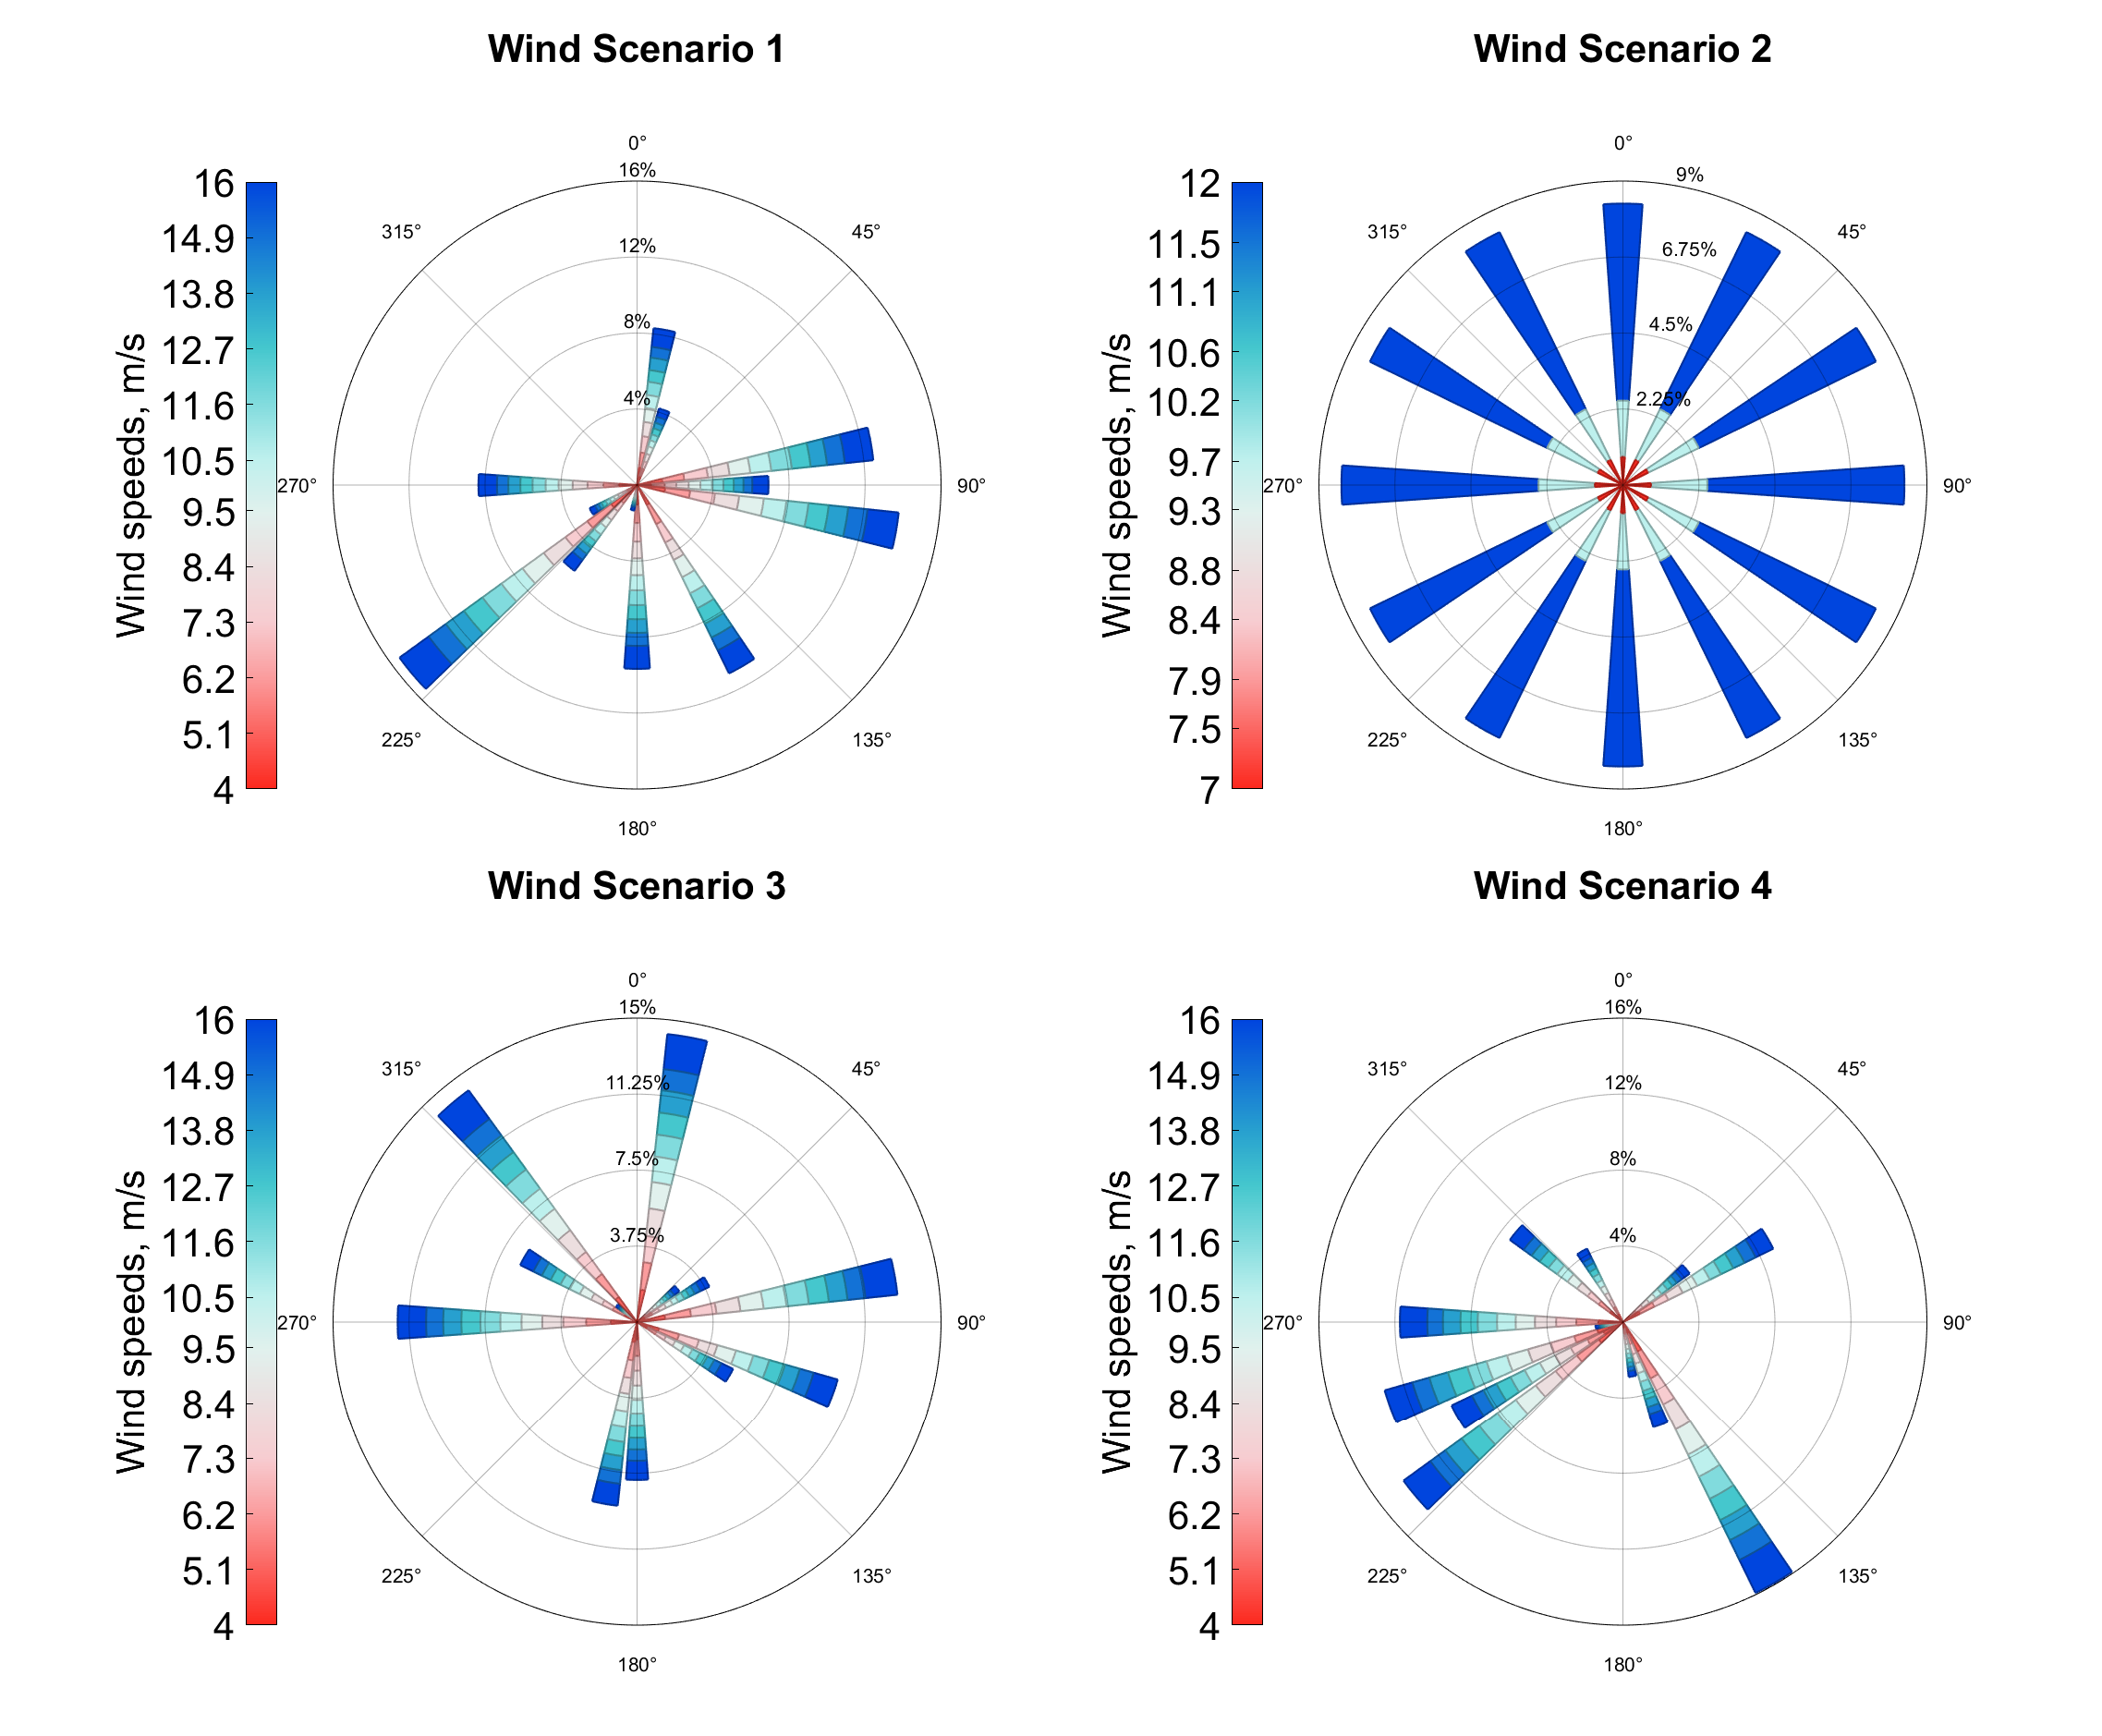
\includegraphics[width=1.0\columnwidth]{4ws.eps}
	\caption{Four kinds of wind scenarios rose figure.}
	\label{fig:4ws}
\end{figure}
\begin{table}[htbp]
	\captionsetup{labelfont={color=black},font={color=black}}
	\centering
	\scriptsize
	\caption{The Setup parameters of wind turbines.}
	\resizebox{0.9\textwidth}{!}{
		\begin{tabular}{>{\centering}m{3cm} >{\centering\arraybackslash}m{3cm}}
			\hline
			Parameter & Value \\
			\hline
			Scale of wind farm & 21 $\times$ 21 \\
			Width of grids & 77 $\times$ 3 m \\
			Surface roughness & 0.25 mm \\
			Rotor diameter $r$ & 77 m \\
			Wind turbines height & 80 m \\
			\hline
		\end{tabular}
	}
	\label{turbinedes}
\end{table}
All algorithms in this study optimize the WFLO problem for 30, 35, and 40 wind turbine sizes under four different complex wind scenarios. These four wind scenarios are shown in Fig. \ref{fig:4ws}. Wind scenario 1 (S1) represents a scenario with three wind speeds and twelve wind directions; wind scenario 2 (S2) represents a uniformly distributed scenario with three wind speeds and twelve wind directions; wind scenario 3 (S3) represents a scenario with four wind speeds and twelve wind directions; and wind scenario 4 (S4) represents a scenario with six wind speeds and twelve wind directions. The number of iterations for all algorithms was 200, the population size was 50, and 10 independent non-repeating experiments were performed to eliminate chance. All algorithms are implemented on an experimental platform with Intel (R) Core (TM) i9-12900K 3.90 GHz CPU, 32 GB of RAM, GPU RTX 3090, and 24 GB of video memory.

\subsection{Analysis of results for wind scenarios}
\begin{table*}
	\captionsetup{labelfont={color=black},font={color=black}}
	\centering
	\caption{The Conversion efficiency ($\%$) of the algorithm for four wind scenarios and three turbine scales.}
	\label{table:dataset}
	\begin{adjustwidth}{-4.2cm}{}
	\resizebox{1.7\textwidth}{!}{
		\begin{tabular}{l|lllll|c|lllll}\hline
			& & TN30    & TN35   & TN40  & $p$-value    & & &TN30    & TN35   & TN40  & $p$-value  \\\hline
			\multirow{13}{*}{\rotatebox[origin=c]{90}{Wind scenario 1}} & AGA  & 95.58 (±0.16)  & 94.16 (±0.22)  & 92.87 (±0.19)  & 9.77E-04   &\multirow{13}{*}{\rotatebox[origin=c]{90}{Wind scenario 2}}& AGA  & 95.01 (±0.26)  & 93.41 (±0.26)  & 92.01 (±0.28) &9.77E-04   \\
			& IntGA  & 93.87 (±0.51)  &92.65 (±0.67)  & 91.05 (±0.31)  & 9.77E-04  & &IntGA  & 94.66 (±0.68)  & 92.76 (±0.88)  & 91.40 (±0.38)&9.77E-04    \\
			& HGSA  & 94.94 (±0.09)  & 93.77 (±0.21)  & 92.48 (±0.28)  &9.77E-04   & &HGSA  & 93.55 (±0.21)  & 91.76 (±0.29)  & 89.78 (±0.24)&9.77E-04    \\
			& BSA  & 95.87 (±0.37)  & 94.39 (±0.46)  & 93.11 (±0.43)  &9.77E-04   & &BSA  & 94.51 (±0.49)  & 92.71 (±0.54)  & 91.20 (±0.43)&9.77E-04    \\
			& ALGSA  & 94.57 (±0.21)  & 94.31 (±0.28)  & 92.52 (±0.29)  & 9.77E-04   & &ALGSA  & 94.01 (±0.42)  & 92.36 (±0.32)  & 89.72 (±0.28)&9.77E-04    \\
			& IWO  & 93.28 (±0.16)  & 91.70 (±0.21)  & 90.32 (±0.17)  &9.77E-04    & &IWO  & 91.92 (±0.21)  & 90.35 (±0.34)  & 88.41 (±0.37)&9.77E-04    \\
			& CJADE  & 96.05 (±0.36)  & 94.65 (±0.00)  & 93.15 (±0.00)  &9.77E-04    & &CJADE  & 95.26 (±0.14)  & 93.46 (±0.26)  & 91.35 (±0.00)&9.77E-04    \\
			& LSHADE$_S$  & 97.48 (±0.24)  & 96.29 (±0.21)  & 94.78 (±0.24)  &1.95E-03    & &LSHADE$_S$  & 96.81 (±0.42)  & 95.36 (±0.20)  & 94.00 (±0.36)&9.77E-04    \\
			& AGPSO  & \underline{97.53 (±0.19)}  & 96.15 (±0.19)  & \underline{95.32 (±0.32)}  &9.77E-04   & &AGPSO  & \underline{97.26 (±0.36)}  & 95.85 (±0.21)  & 94.40 (±0.21)&9.77E-04    \\
			& CLPSO  & 93.61 (±0.13)  & 91.67 (±0.00)  & 90.18 (±0.03)  &9.77E-04   & &CLPSO  & 91.62 (±0.36)  & 89.80 (±0.04)  & 87.63 (±0.00)&9.77E-04    \\
			& GLPSO  & 97.48 (±0.21)  & \underline{96.43 (±0.18)}  & 95.23 (±0.34)  &9.77E-04    & &GLPSO  & 97.15 (±0.14)  & 95.91 (±0.27)  & 94.26 (±0.32) &9.77E-04   \\
			& CGPSO  & 97.51 (±0.26)  & 96.32 (±0.20)  & 95.13 (±0.20)  &9.77E-04    & &CGPSO  & 97.19 (±0.20)  & \underline{95.93 (±0.24)}  & \underline{94.42 (±0.22)}&9.77E-04    \\
			& RPSO  &\textbf{98.17 (±0.18)}  &\textbf{97.21 (±0.44)}  & 	\textbf{95.83 (±0.31)}  & \quad$--$     & &RPSO  & \textbf{97.77 (±0.30)}  & \textbf{96.71 (±0.34)}  & \textbf{95.06 (±0.31)} &\quad$--$    \\\hline
			
			\multirow{13}{*}{\rotatebox[origin=c]{90}{Wind scenario 3}} & AGA  & 96.10 (±0.11)  & 95.10 (±0.13)  & 94.00 (±0.11)  & 9.77E-04   &\multirow{13}{*}{\rotatebox[origin=c]{90}{Wind scenario 4}}& AGA  & 96.94 (±0.15)  & 96.04 (±0.11)  & 95.05 (±0.20)&9.77E-04    \\
			& IntGA  & 95.10 (±0.35)  & 94.02 (±0.39)  & 92.67 (±0.43)  &9.77E-04   & &IntGA  & 95.78 (±0.37)  & 94.46 (±0.37)  & 93.40 (±0.68) &9.77E-04   \\
			& HGSA  & 95.94 (±0.17)  & 94.70 (±0.14)  & 93.56 (±0.17)  &9.77E-04   & &HGSA  & 96.40 (±0.20)  & 95.12 (±0.15)  & 94.02 (±0.24)&9.77E-04    \\
			& BSA  & 96.27 (±0.20)  & 95.37 (±0.32)  & 94.15 (±0.22) &9.77E-04  & &BSA  & 96.91 (±0.28)  & 95.65 (±0.51)  & 94.71 (±0.35)&9.77E-04    \\
			& ALGSA  & 96.20 (±0.27)  & 95.07 (±0.17)  & 93.44 (±0.26)  &9.77E-04    & &ALGSA  & 96.41 (±0.19)  & 95.08 (±0.30)  & 93.89 (±0.27)&9.77E-04  \\
			& IWO  & 94.61 (±0.23)  & 93.36 (±0.14)  & 92.11 (±0.07)  &9.77E-04    & &IWO  & 95.20 (±0.17)  & 94.02 (±0.17)  & 92.92 (±0.21)&9.77E-04    \\
			& CJADE  & 96.71 (±0.17)  & 95.47 (±0.13)  & 94.14 (±0.01)  &9.77E-04    & &CJADE  & 96.94 (±0.08)  & 96.09 (±0.11)  & 94.96 (±0.22)&9.77E-04    \\
			& LSHADE$_S$  & 97.37 (±0.08)  & 96.39 (±0.13)  & 95.38 (±0.24)  &9.77E-04    & &LSHADE$_S$  & 98.28 (±0.26)  & \underline{97.59 (±0.23)}  & 96.85 (±0.26)&9.77E-04    \\
			& AGPSO  & 97.47 (±0.12)  & 96.54 (±0.13)  & 95.55 (±0.16)  &9.77E-04    & &AGPSO  & 98.29 (±0.14)  & 97.55 (±0.21)  & 96.94 (±0.24) &9.77E-04   \\
			& CLPSO  & 94.53 (±0.17)  & 93.43 (±0.09)  & 91.69 (±0.13)  &9.77E-04    & &CLPSO  & 95.06 (±0.17)  & 93.47 (±0.36)  & 92.46 (±0.08)&9.77E-04    \\
			& GLPSO  & 97.48 (±0.14)  & \underline{96.58 (±0.13)}  & 95.53 (±0.13)  &9.77E-04    & &GLPSO  & 98.14 (±0.20)  & 97.49 (±0.16)  & \underline{97.01 (±0.23)} &9.77E-04   \\
			& CGPSO  & \underline{97.48 (±0.12)}  & 96.52 (±0.09)  & \underline{95.64 (±0.17)}  &9.77E-04    & &CGPSO  & \underline{98.33 (±0.11)}  & 97.57 (±0.29)  & 96.85 (±0.20)&9.77E-04    \\
			& RPSO  & \textbf{97.82 (±0.06)}  & \textbf{97.07 (±0.21)}  & \textbf{95.90 (±0.31)}  &\quad$--$    & &RPSO  & \textbf{98.68 (±0.14)}  & \textbf{98.14 (±0.17)}  & \textbf{97.33 (±0.41)}&\quad$--$    \\\hline	
\end{tabular}}
\end{adjustwidth}
\end{table*}
\begin{table}[t]
	\centering
	\arrayrulecolor{blue}
	\begin{adjustwidth}{-2cm}{}
	\begin{tabular}{|c|c|c|c|}
		\hline
		\textbf{parameters} & \textbf{First-order sensitivity(S1)} & \textbf{Total-order sensitivity(ST)} & \textbf{Second-order interactions(S2)} \\
		\hline
		Wind\_C & 0.1097 & 0.1860 & Wind\_C - Turbines: 0.0055 \\
		\hline
		Turbines & 0.1400 & 0.1301 & Wind\_C - Algorithms: 0.1005 \\
		\hline
		Algorithms & 0.6695 & 0.7325 & Turbines - Algorithms: -0.0184 \\
		\hline
	\end{tabular}
	\end{adjustwidth}
	\caption{\textcolor{blue}{Sensitivity analysis of each hyper-parameter using variance decomposition (Sobol).}}
	\label{tab:sobol_sensitivity}
\end{table}
\begin{figure}
	\centering
	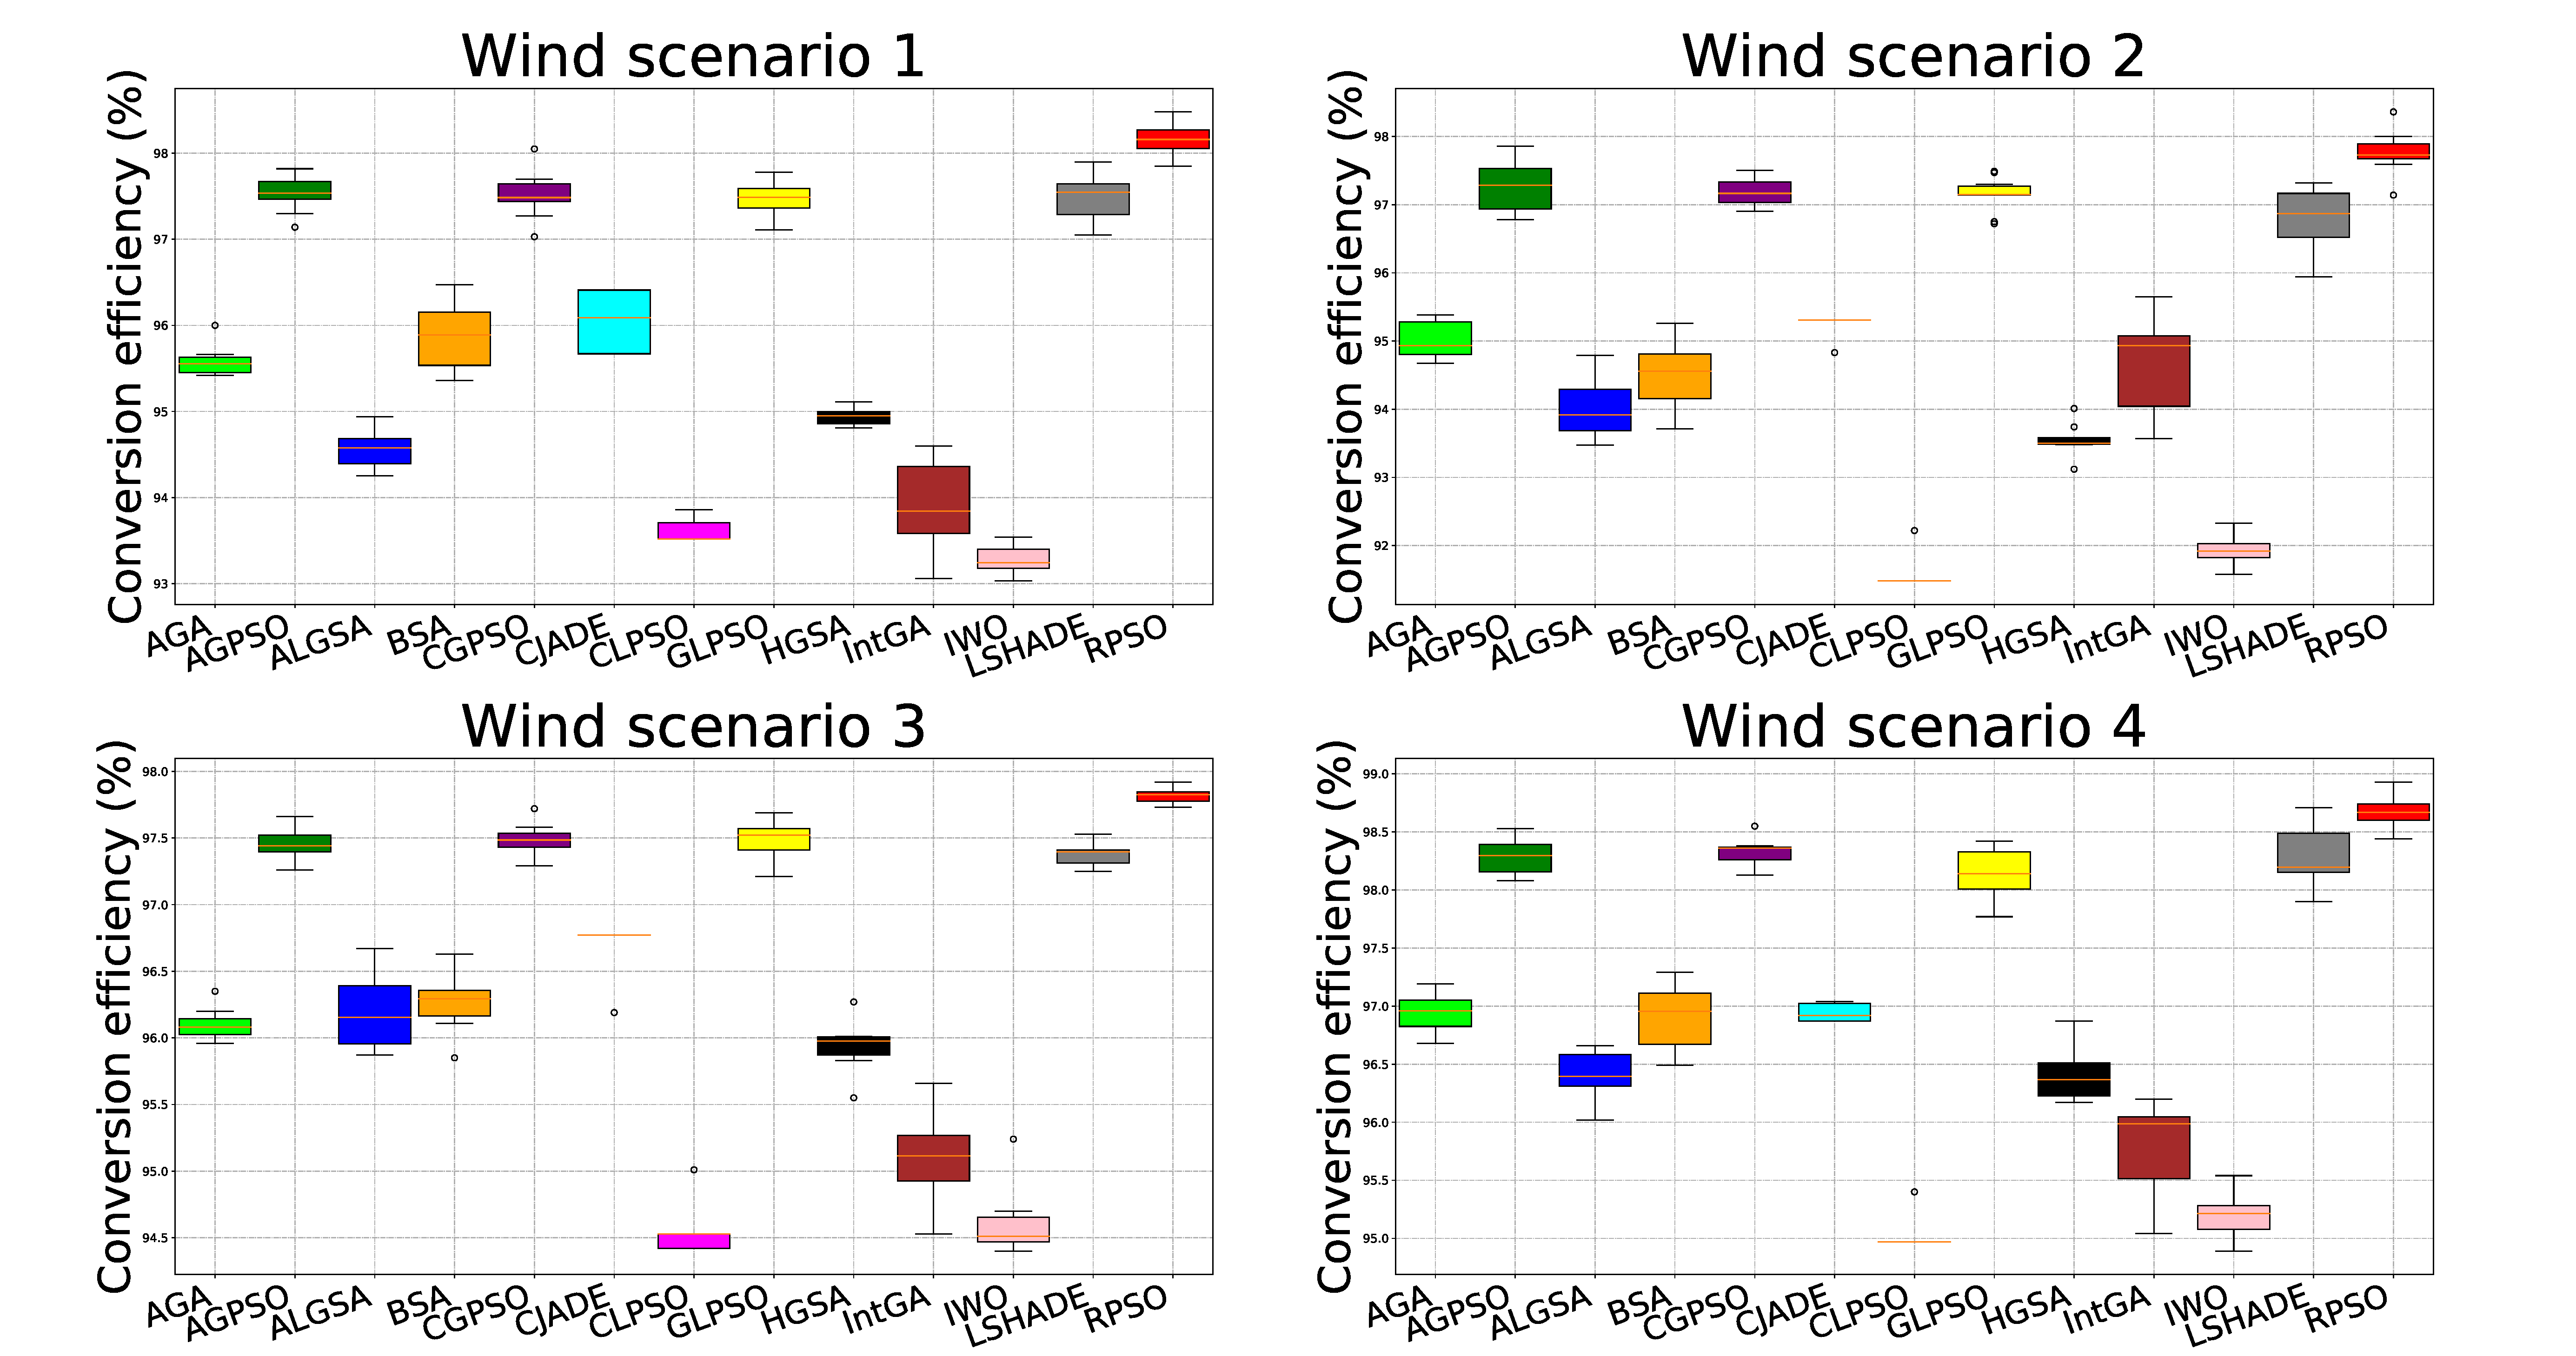
\includegraphics[width=1\textwidth]{4box.eps}
	\caption{Box figures of all algorithms for four wind scenarios.}
	\label{fig:4box}
\end{figure}
\begin{figure*}
	\centering
	\hspace*{-3cm}
	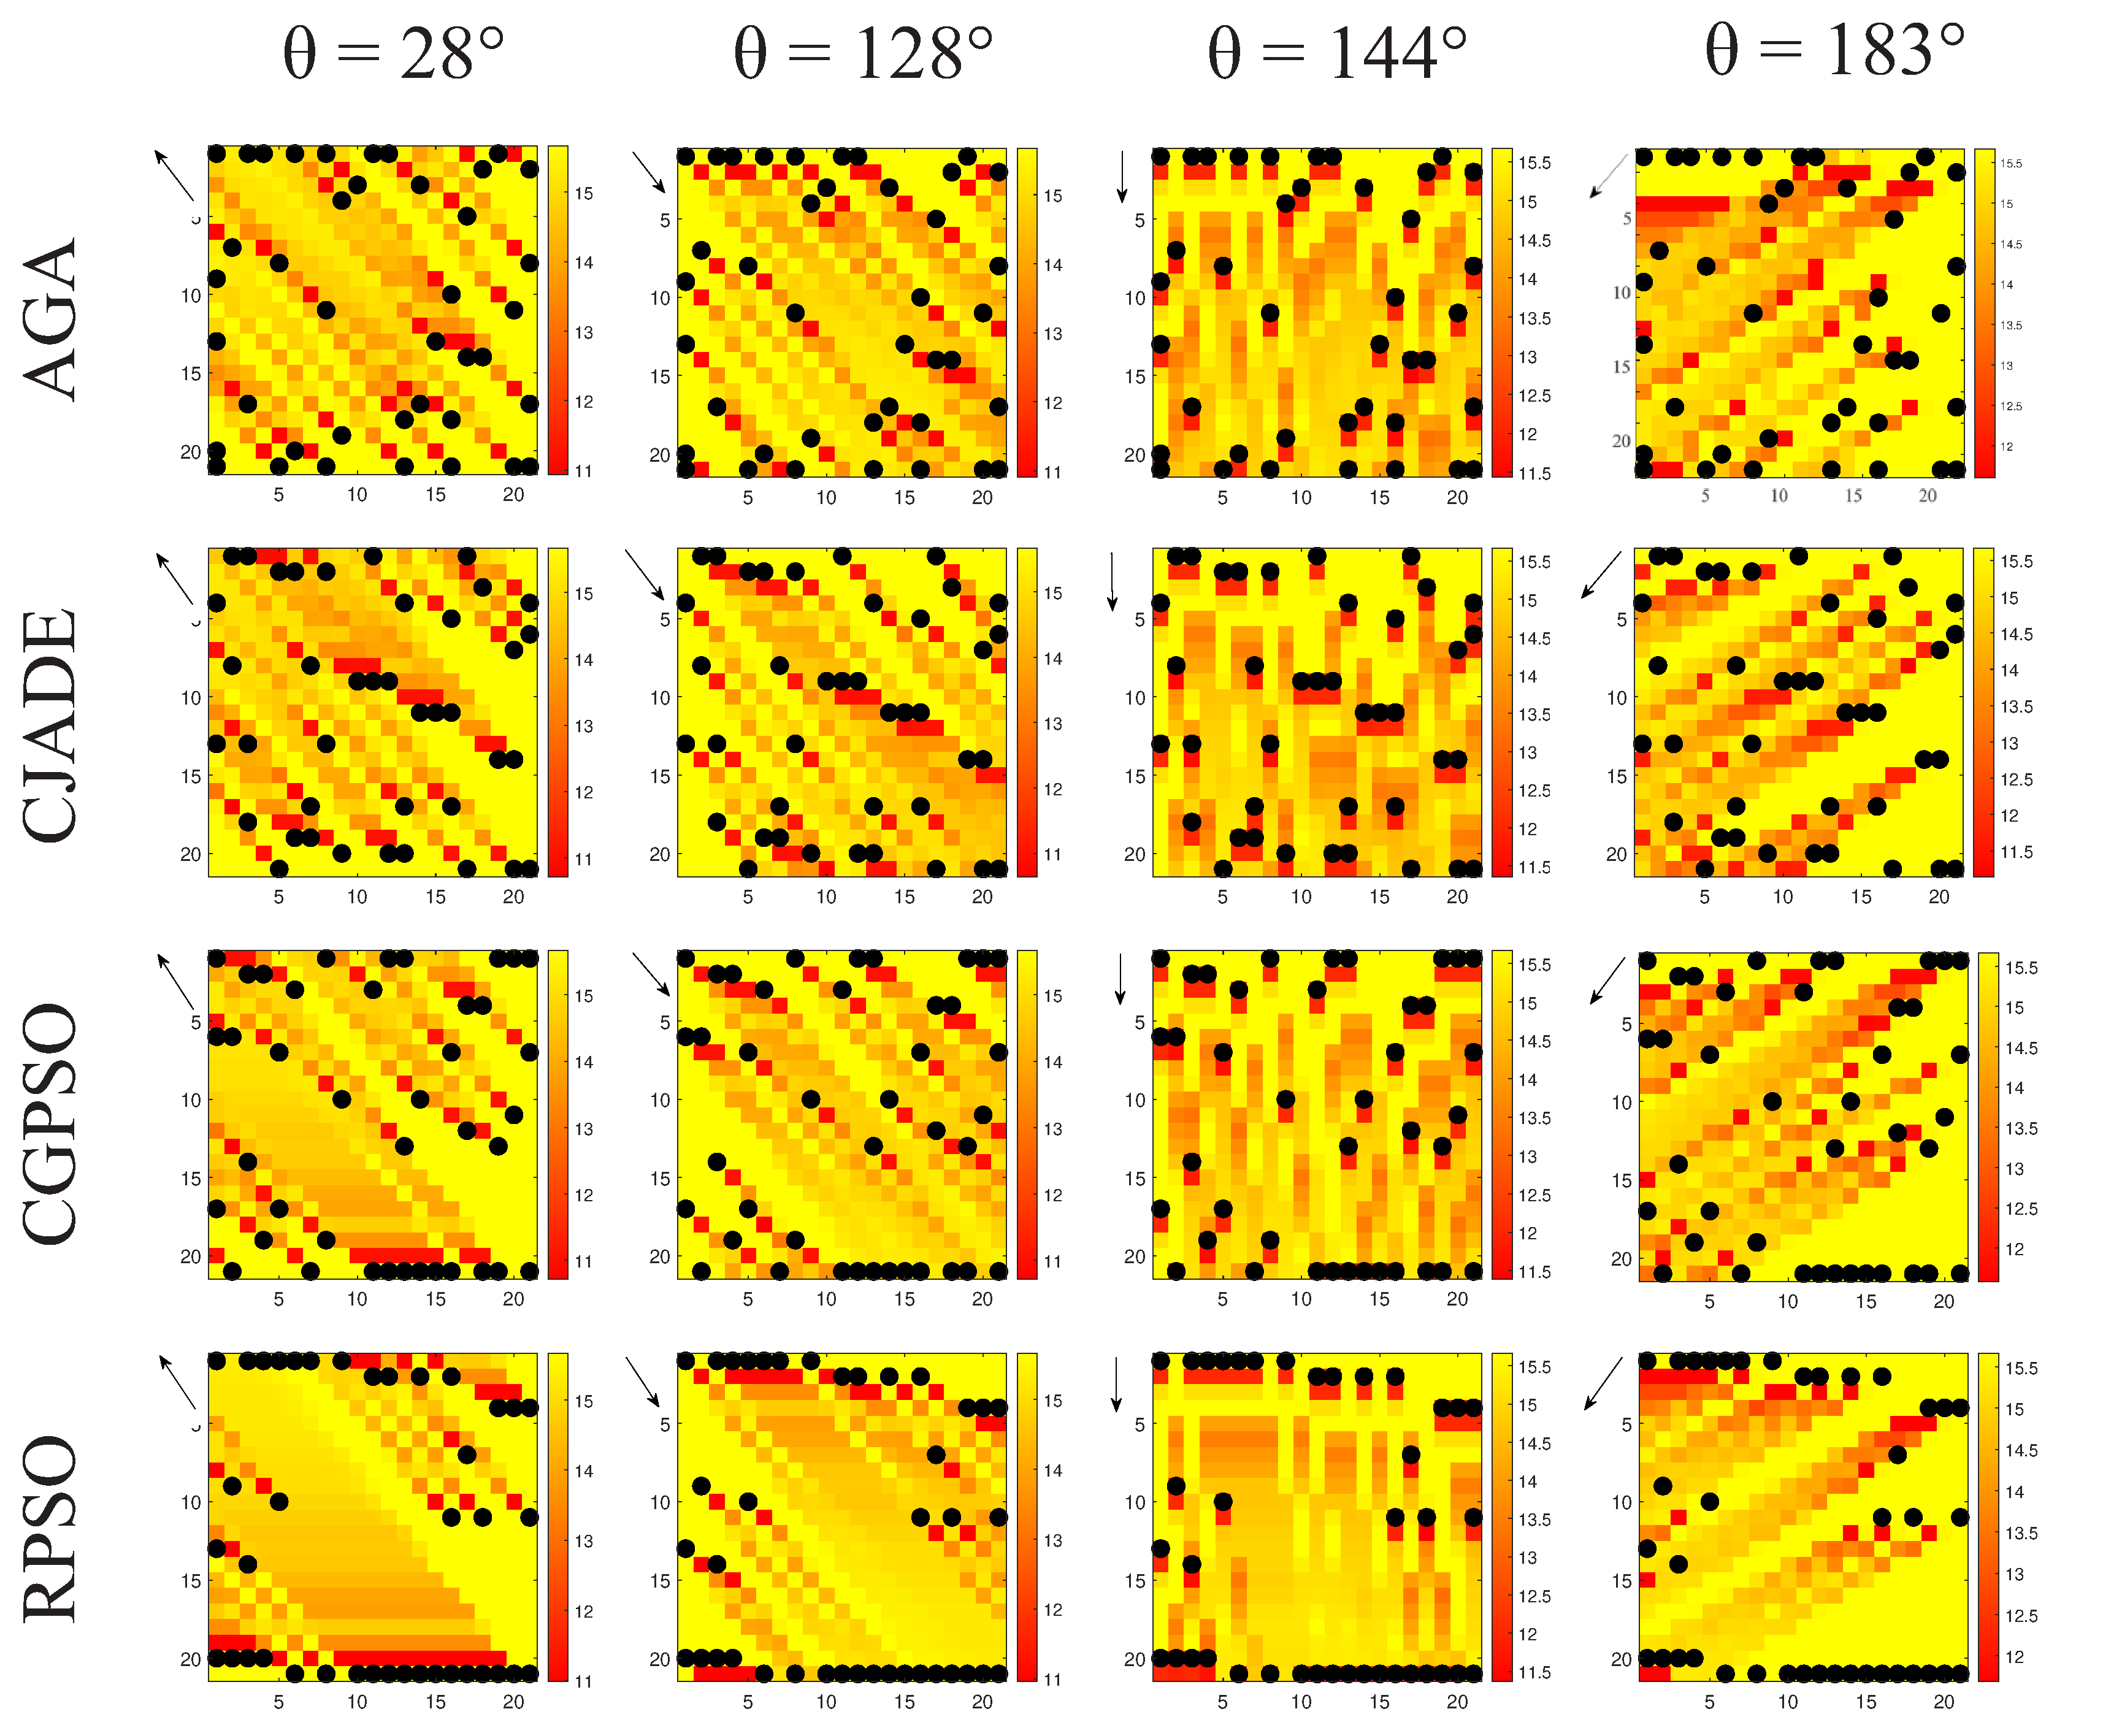
\includegraphics[width=1.5\textwidth]{layout.eps}
	\caption{The layouts of four algorithms with wake attenuation under four wind directions. The black dot represents the turbine and the red to yellow color blocks indicate low to high wind speeds at that point.}
	\label{fig:layout}
\end{figure*}
Table \ref{table:dataset} enumerates the conversion efficiencies of all algorithms across four wind scenarios, considering three turbine sizes positioned at 30, 35, and 40. The conversion efficiencies are determined using Eq. \eqref{eta}. The numbers in parentheses denote the standard deviation of the results obtained from all independent and unrepeated experiments. Additionally, we conducted the Wilcoxon signed-rank test for each algorithm, yielding a $p$-value less than 0.05. It is evident that the proposed RPSO algorithm consistently achieves the highest conversion efficiency across all scenarios. Additionally, the underlined entries in the figure represent the second-highest experimental results. Moreover, the figure illustrates that the enhanced variants of PSO, namely CGPSO, GLPSO, and AGPSO, perform admirably in addressing the WFLO problem. \textcolor{blue}{In addition, we have done a sensitivity analysis of the algorithm's performance for various parameter scenarios. As shown in Table \ref{tab:sobol_sensitivity}, the first-order sensitivity index (S1) means the contribution of each parameter independently to the result. Total effect sensitivity index (ST) means the total contribution of each parameter and its interaction with other parameters to the results. Second-order interaction effects (S2) means the contribution to the results of the interactions between the parameters, listing only the meaningful interaction terms. From the data in the table, it can be seen that algorithm is the dominant factor affecting the results, accounting for 73.25$\%$ of the total effect, indicating that the choice of different algorithms has the most significant effect on the final results. Wind condition and turbine count have a smaller effect, but wind condition shows a smaller effect when combined with the algorithm combination showed some interaction effect, which suggests that different algorithms may have different effects under different wind conditions. Turbine count has a lower total contribution and almost no interaction effect, suggesting that it plays a smaller role in the output.}
\begin{figure}
	\centering
	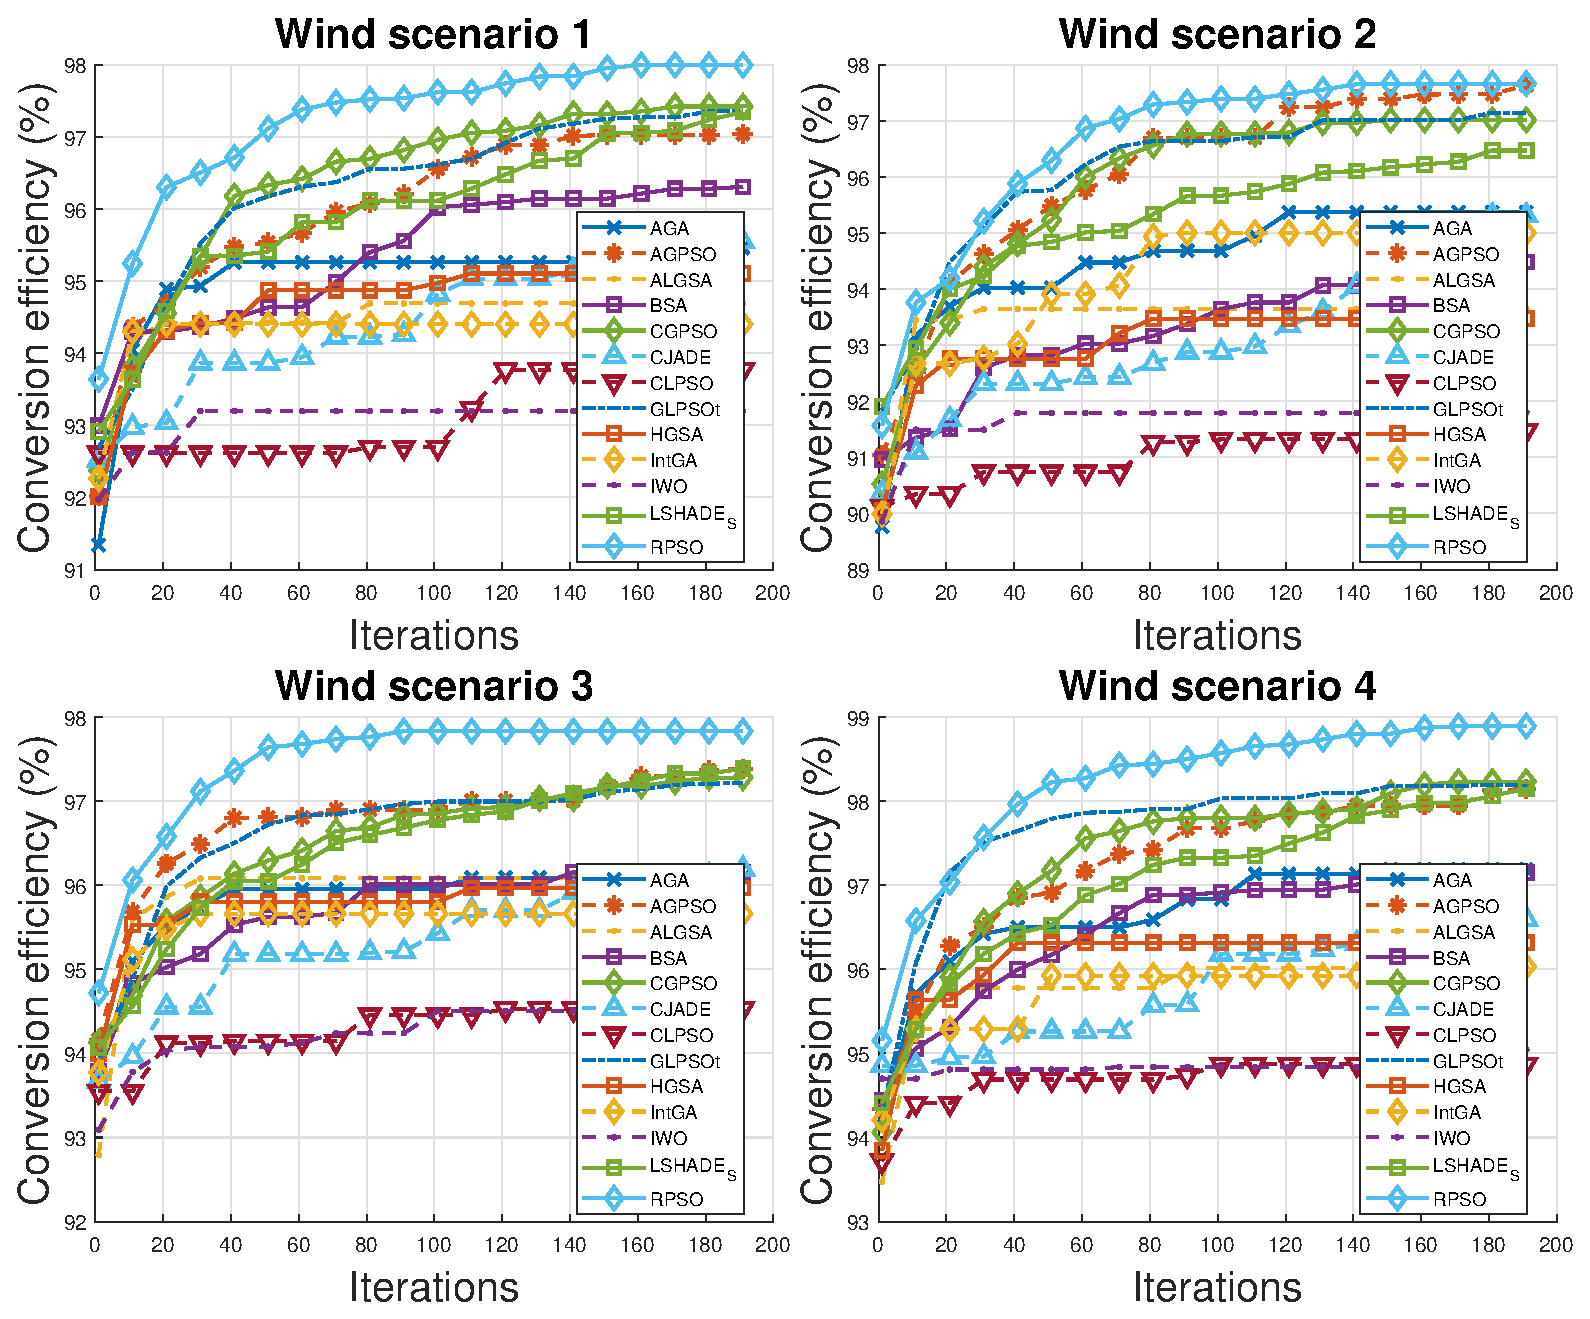
\includegraphics[width=1\columnwidth]{4conv.eps}
	\caption{Convergence figures of all algorithms for four wind scenarios.}
	\label{fig:4conv}
\end{figure}

The stability of all algorithms is depicted in Fig. \ref{fig:4box}. Notably, the proposed RPSO algorithm achieves the highest conversion efficiency while maintaining results within a relatively stable range across experiments, exhibiting minimal fluctuations and variability. Fig. \ref{fig:4conv} illustrates the convergence behavior of all algorithms 200 iterations for four wind scenarios. In all scenarios, RPSO consistently outperforms other algorithms, exhibiting significant improvement from the first 20 iterations onward. However, in scenarios S2 and S4, similar convergence values are observed with GLPSO around the 20th iteration. This occurrence could be attributed to the standardized nature of S2 and the increased complexity of S4, which features 6 wind speeds and 12 wind directions, introducing higher levels of stochasticity compared to other scenarios.

Fig. \ref{fig:layout} illustrates the distribution of selected algorithms across four wind angles under scenario S4, showcasing their response to wake effects. Each black dot in the wind farm denotes a wind turbine, while the color of each region signifies the prevailing wind speed in that area. The majority of regions impacted by wake effects are situated behind the turbines, highlighting the importance of minimizing wake effects on downstream turbines to address this challenge effectively. Examining the distribution, it's evident that many underperforming AGAs are positioned in areas severely affected by wake effects. Conversely, RPSOs are strategically located on both sides of the wind field in a linear arrangement, potentially minimizing the impact of wake effects on downstream turbines. This strategic placement underscores the efficacy of RPSO in optimizing turbine layout to mitigate wake effects and enhance overall performance.

\subsection{Analysis of RL}
We first analyze the results produced by RPSO through the distribution and convergence plots of the new weights $W_{\alpha}$ and $W_{\beta}$. Subsequently, to further validate the effectiveness of RL, we compare the performance of the algorithm without RL through ablation experiments.
\subsubsection{Analysis of distribution of results}
\begin{figure}[!t]
	\centering
	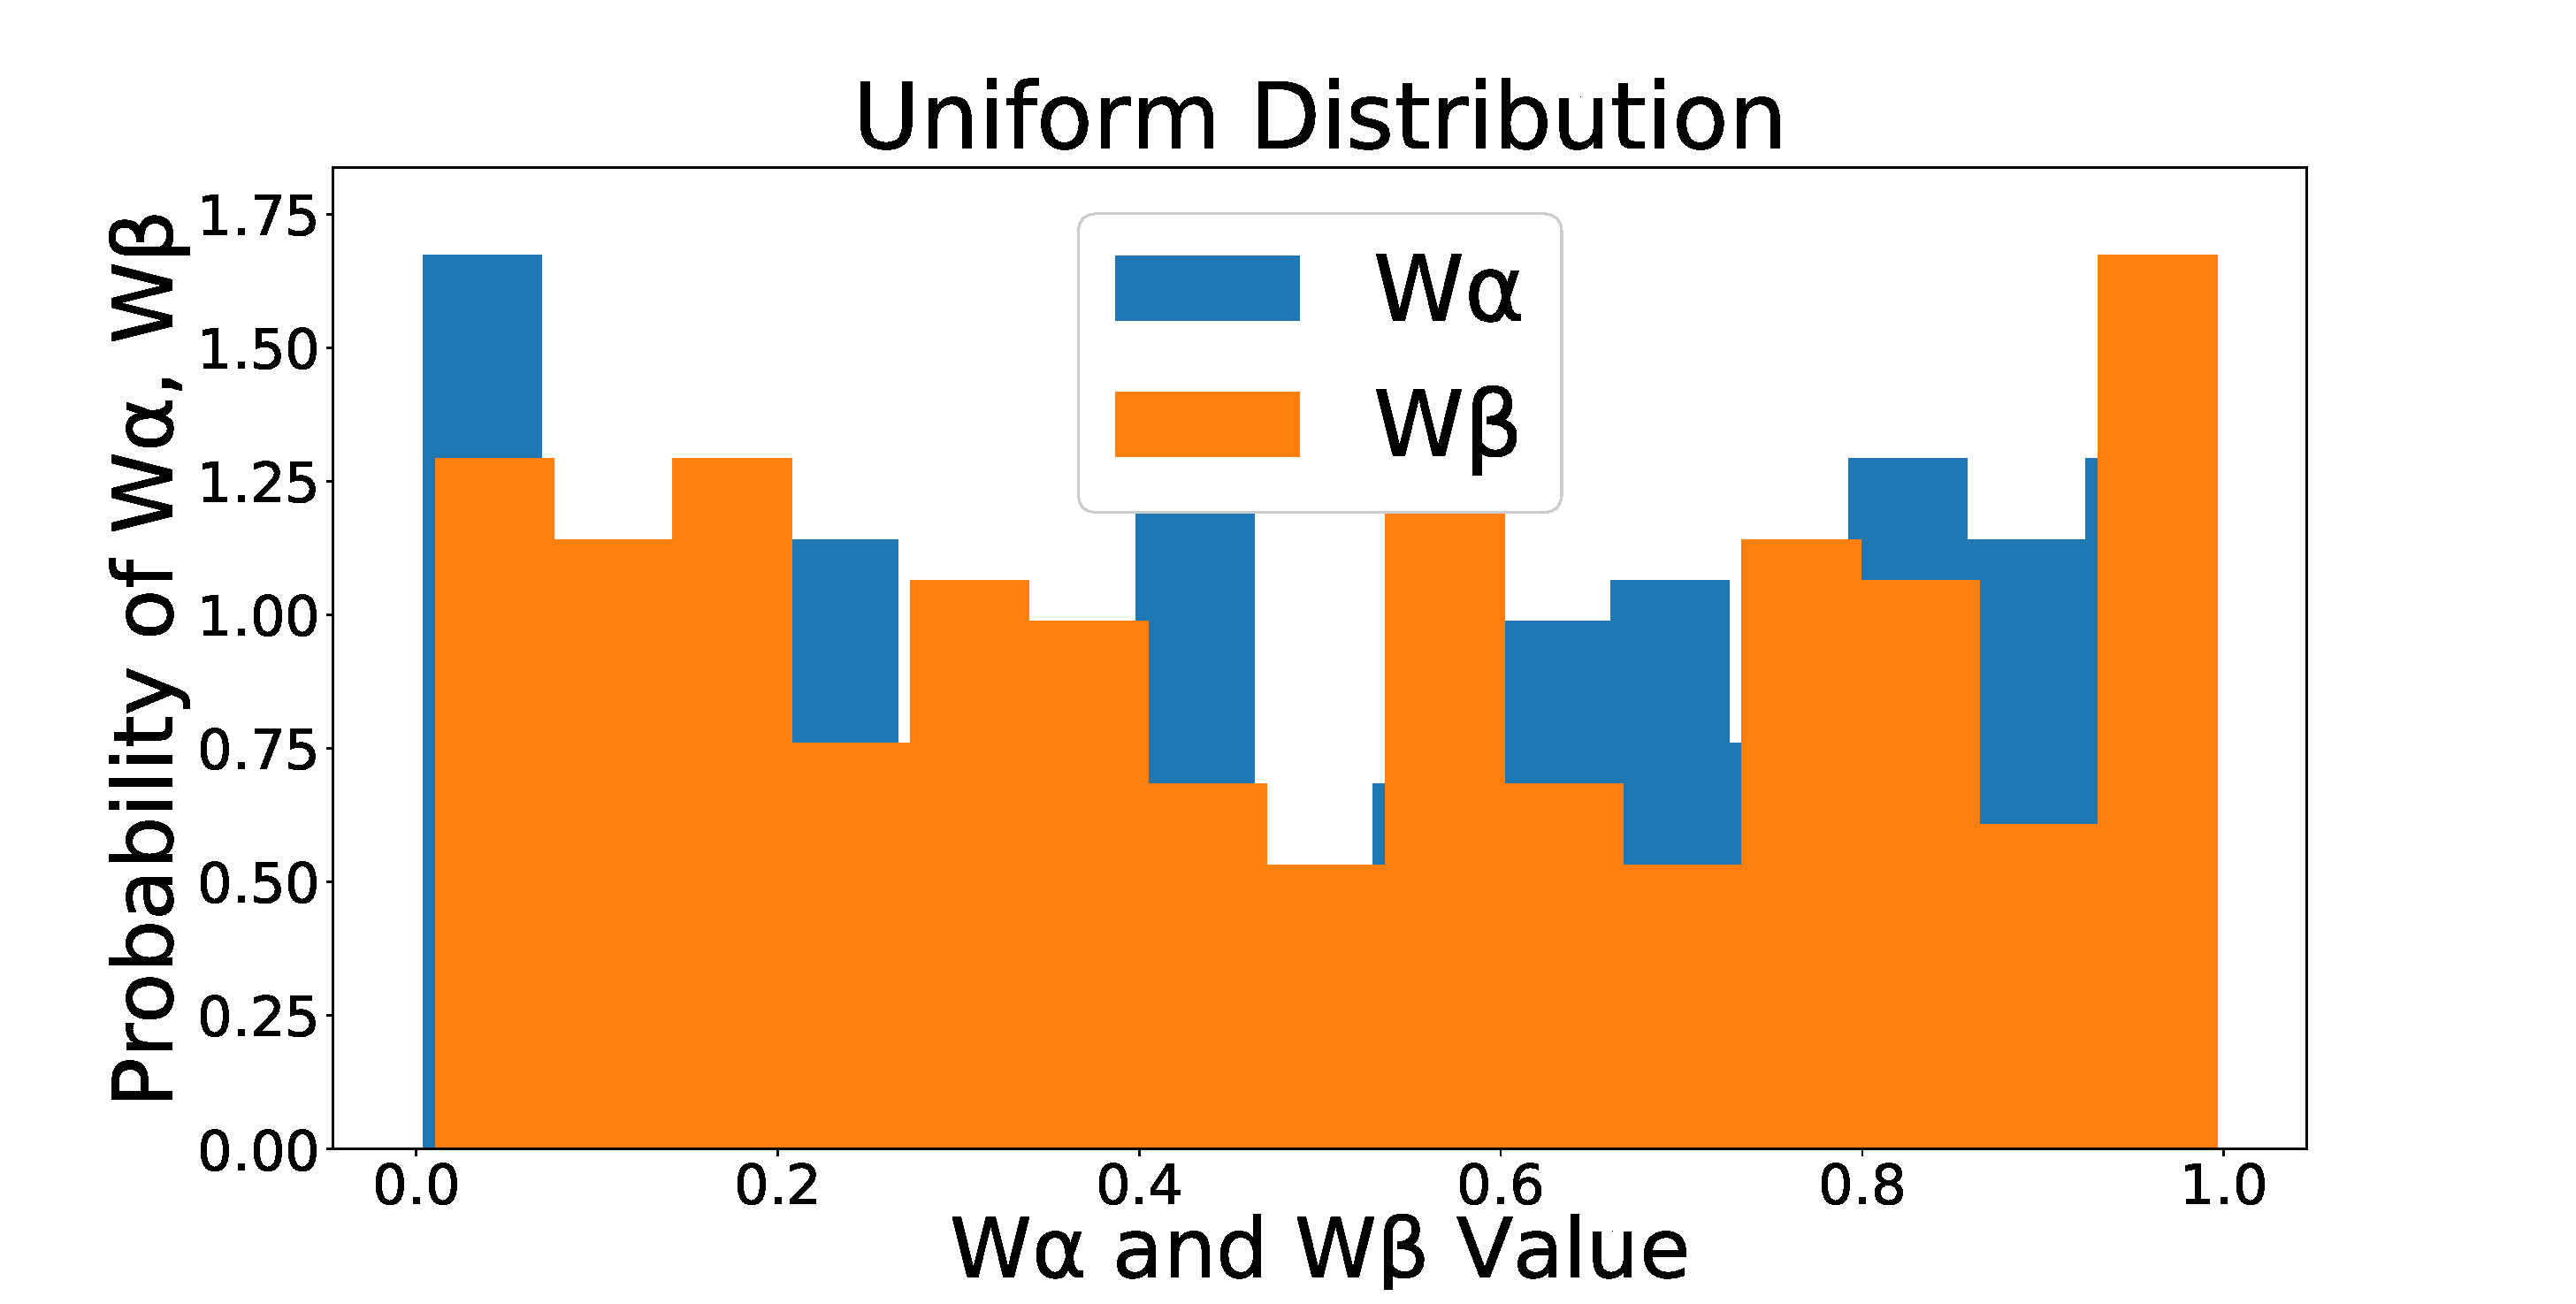
\includegraphics[width=0.6\textwidth]{distribution_uniform.eps}
	\caption{Uniform distribution.}
	\label{fig:uniform}
\end{figure}
In the original work, $r^{\prime}$ is obeying a uniform distribution from 0 to 1. Its probability density function can be expressed as follows:
\begin{align}
	\label{rdistribution}
	prob(r^{\prime})=\begin{cases}
		1, & \text{if}\quad 0 \leq r^{\prime} \leq 1 \\
		0. & \text{otherwise}
	\end{cases}
\end{align}

The probability that any value $r^{\prime}$ is taken in the interval $[0, 1]$ is equal, i.e., the probability density function is constant. The distribution is shown in Fig. \ref{fig:uniform}, all values are evenly distributed between 0 and 1. By learning from the empirical playback of RL, our defined $W_{\alpha}$ and $W_{\beta}$ are no longer disordered random values, but converge in a more optimal direction by learning historical search information. The portion of the distribution generated by the RPSO is shown in Fig. \ref{fig:4distribution}. The blue square bar represents $W_{\alpha}$ and the orange square bar represents $W_{\beta}$. It can be seen that after RL learning, the value of $W_{\alpha}$ is higher than $W_{\beta}$ in most cases, which can reflect the fact that the effect of $pbest$ on the next generation may be a bit more favorable. The convergence curves of $W_{\alpha}$ and $W_{\beta}$ with the number of iterations are shown in Fig. \ref{fig:r_exp}. Where the green curve represents the original $r^{\prime}$, which floats randomly between 0 and 1, the blue curve represents $W_{\alpha}$, and the orange curve represents $W_{\beta}$. It can be seen that the two weight ratios converge in a specific direction from the initial value, which reflects the guiding role that the empirical information of RL plays in the algorithm.
\begin{remark}
	\emph{In contrast to previous work, we explore the solution space for negative values. It is argued in the higher dimensional space of the PPO that the $gbest$, although acting as a globally optimal particle, does not necessarily have to be additive to the algorithm by a certain weighting, but can also be subtractive. We believe that this represents two different directions of exploration.}
\end{remark}
\subsubsection{Ablation experiment}
To further validate the effectiveness of our proposed RL strategy within the algorithm, we conducted ablation experiments on the PPO algorithm employed in RL. The results of these experiments are presented in Table \ref{norl}. \textcolor{blue}{Fig. \ref{fig:four_images} shows the convergence of the effect of whether or not to use RL on the model algorithm for four wind conditions (30 turbines). As can be seen from the figure, RL enhances the model significantly and plays a constructive role in the whole phase of algorithm convergence, not only speeding up the convergence of the algorithm, but also improving the performance.} No-RL denotes the algorithm after removing the PPO strategy. From the experimental results, it can be seen that the algorithm under the no-RL strategy loses to RPSO in all scenarios and for all turbine sizes. To eliminate chance factors, we conducted the Wilcoxon signed-rank test on the experimental outcomes, revealing that all $p$-values were less than 0.05. RL primarily facilitates the utilization of the experience pool playback strategy within the PSO algorithm, leveraging historical search data to inform the direction of subsequent iterations. Without RL, the original algorithm relies solely on randomness during iteration:
\begin{figure}[!t]
	\centering
	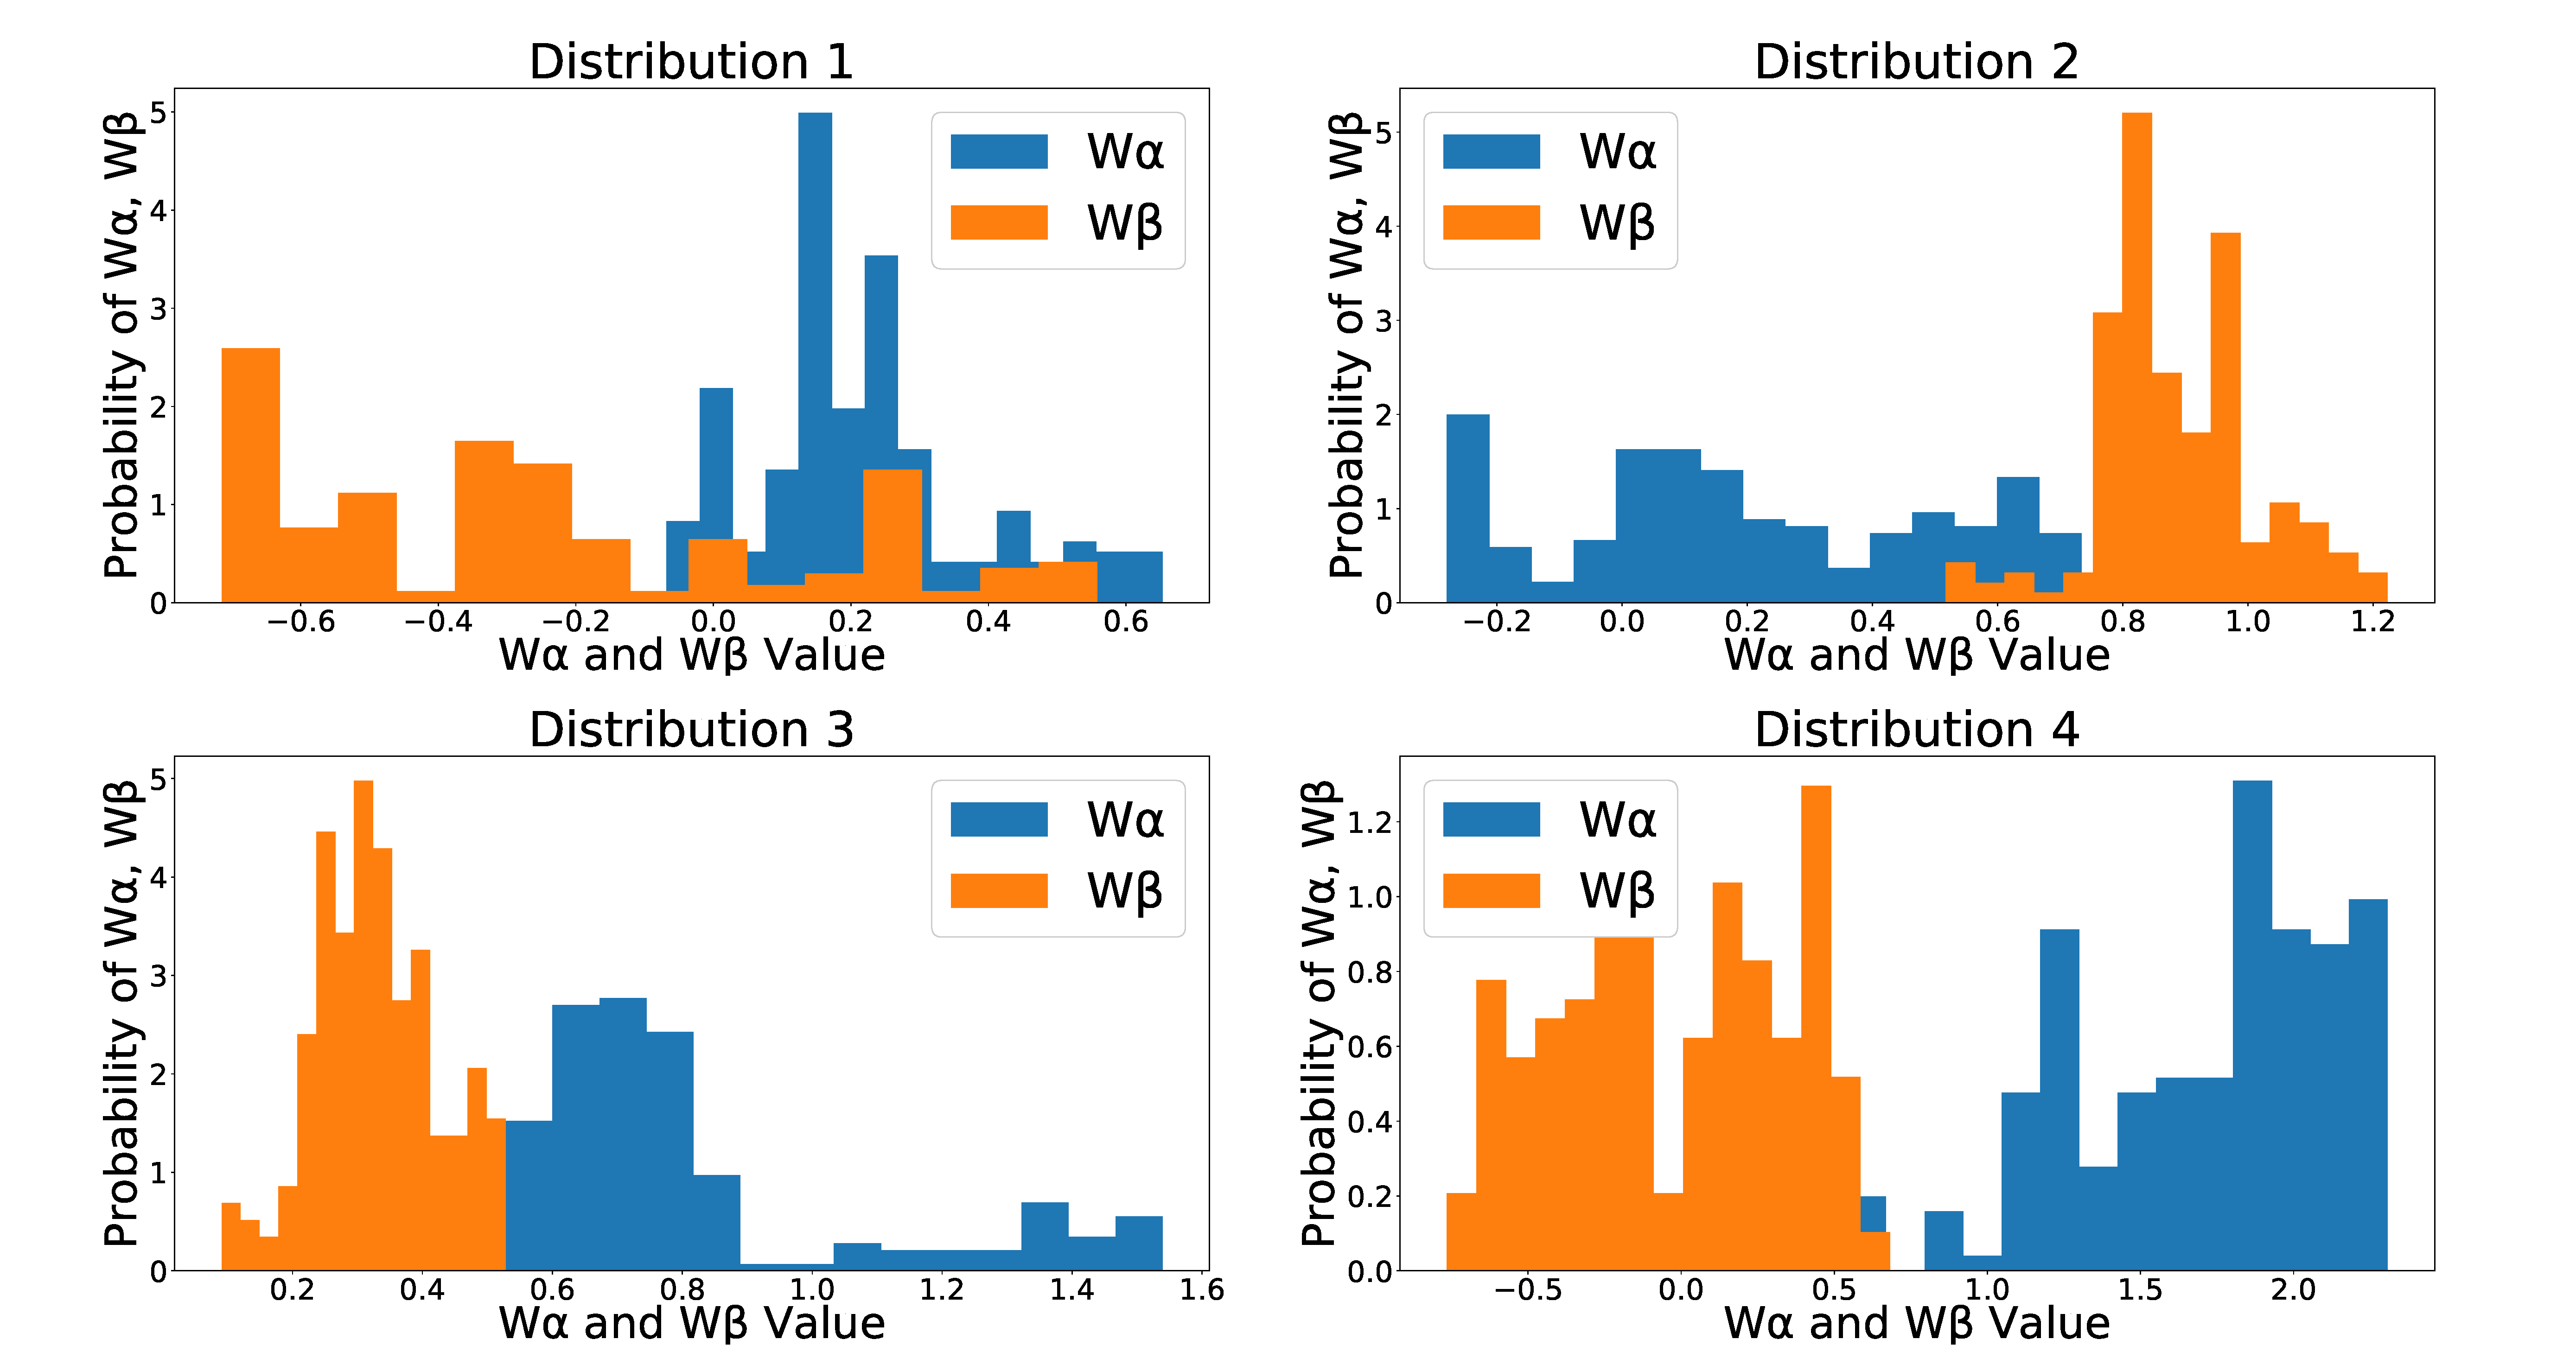
\includegraphics[width=1\textwidth]{4distribution_1pic.eps}
	\caption{Probability distributions of the 4 RPSO species $W_{\alpha}$ and $W_{\beta}$.}
	\label{fig:4distribution}
\end{figure}
\begin{figure}[!t]
	\centering
	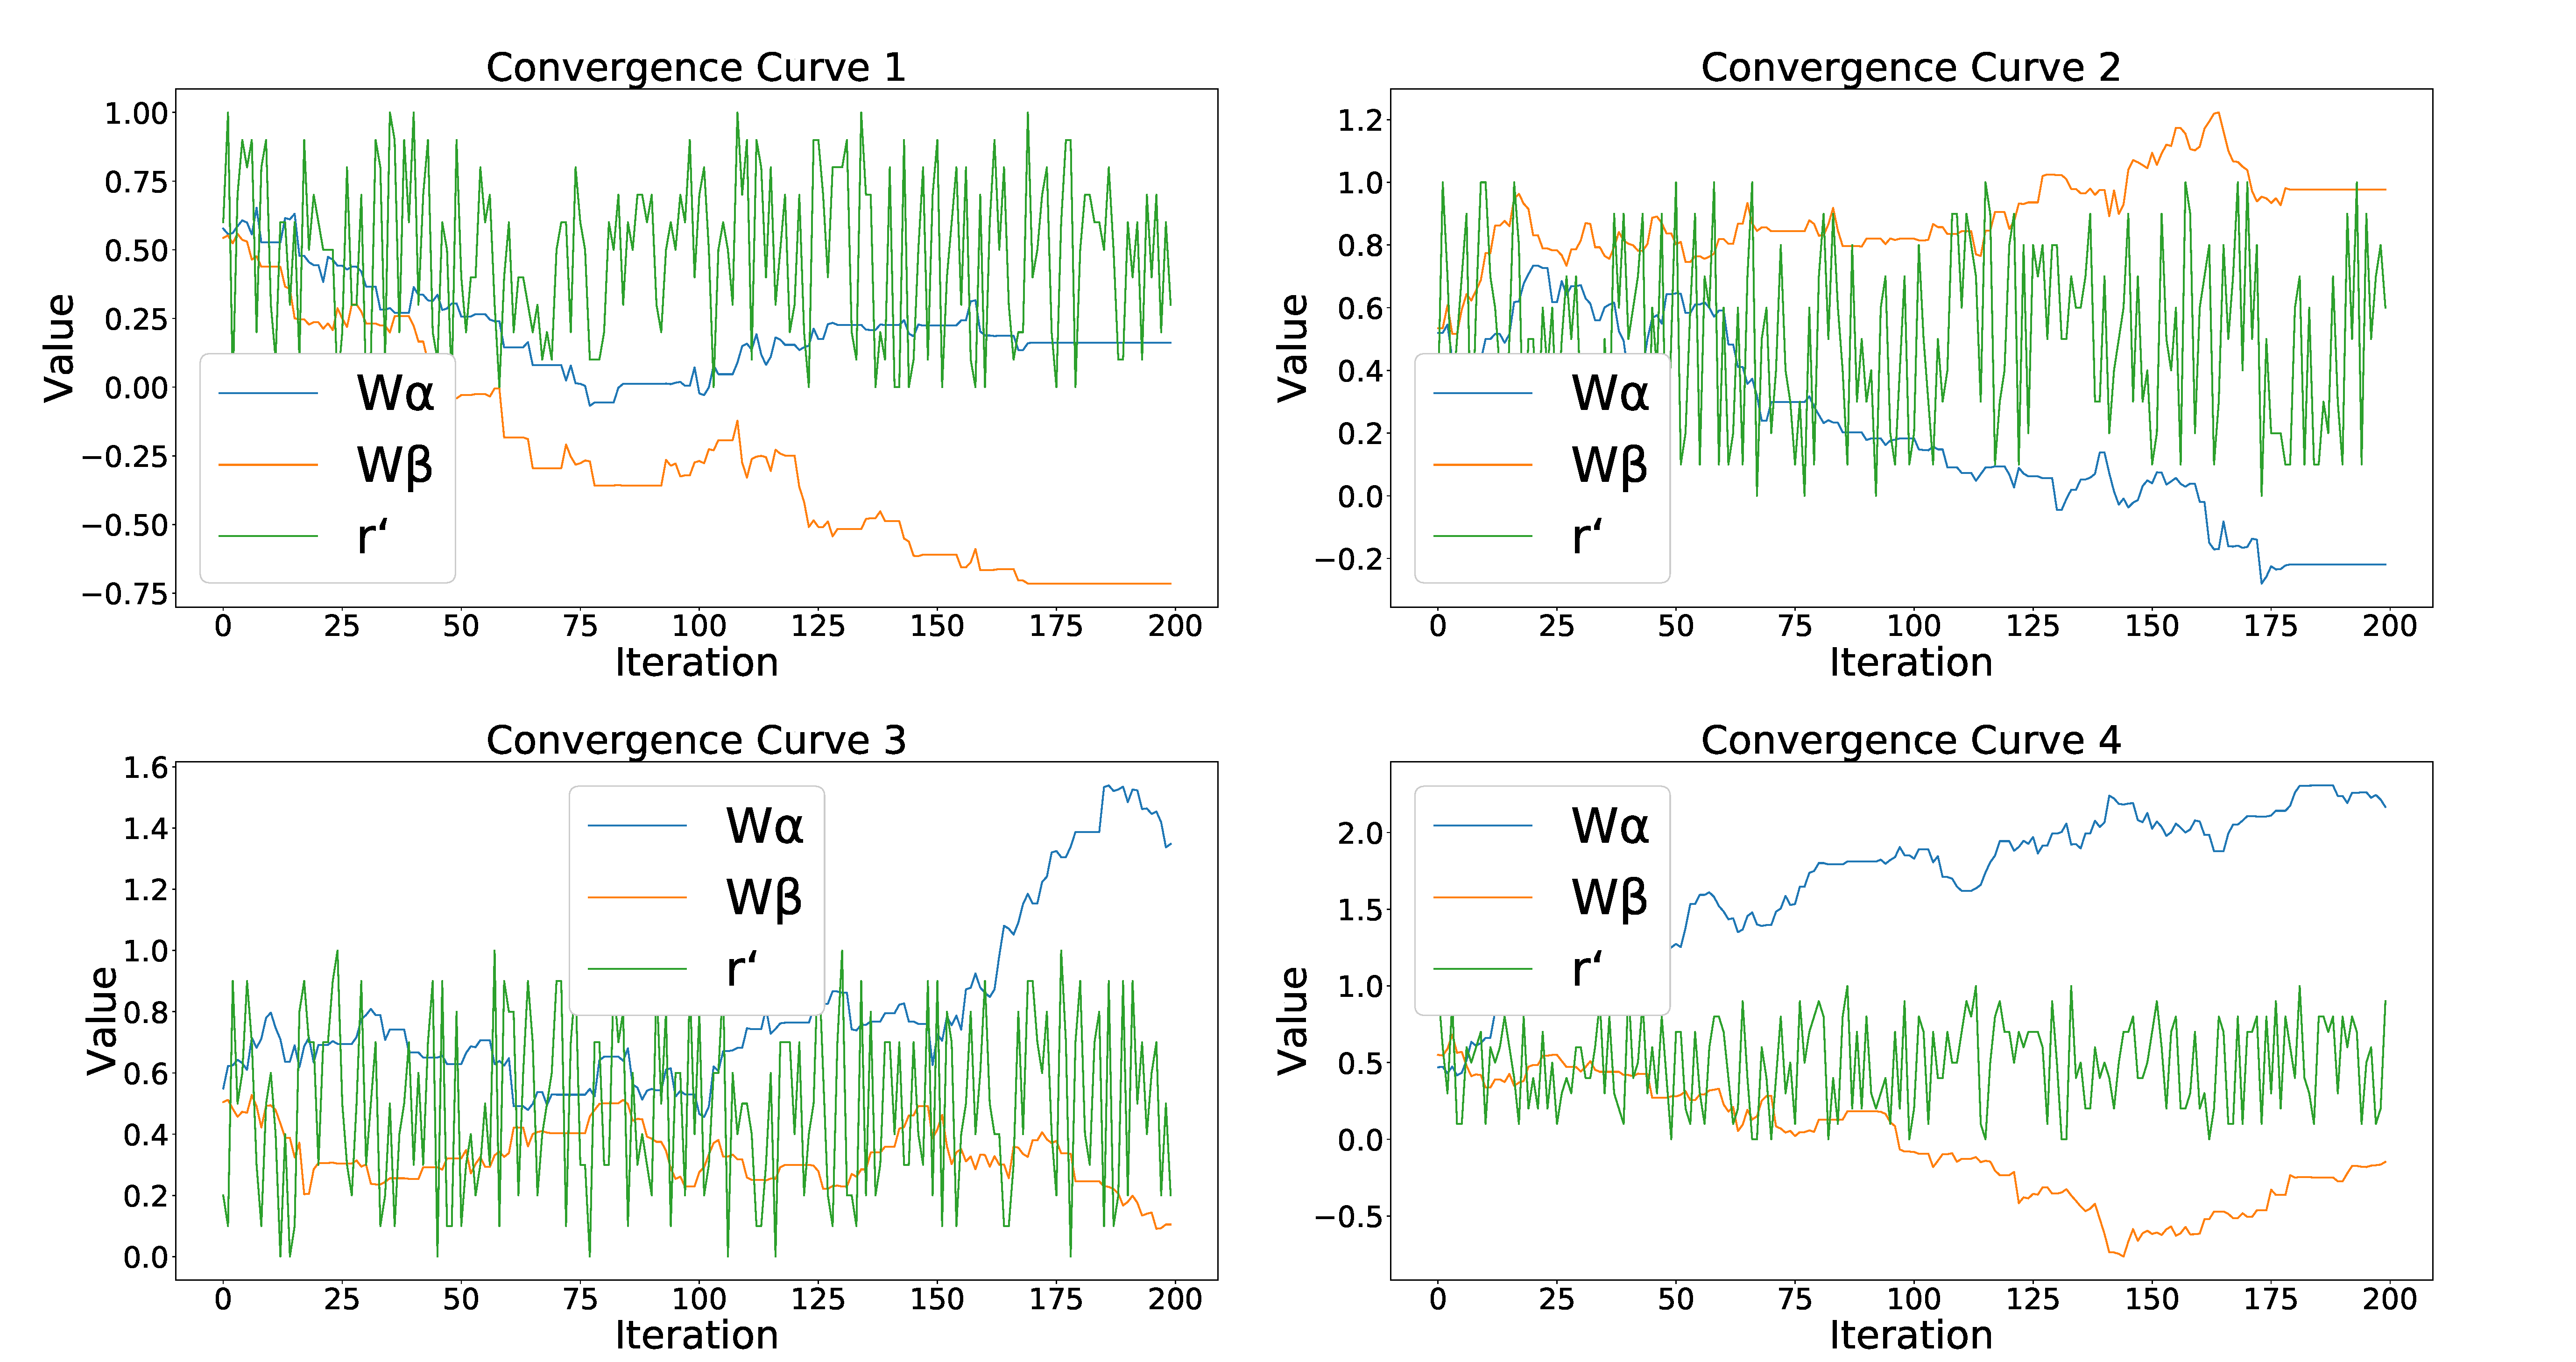
\includegraphics[width=1\textwidth]{r_experiment_1pic.eps}
	\caption{Convergence curves of $W_{\alpha}$ and $W_{\beta}$ with number of iterations.}
	\label{fig:r_exp}
\end{figure}
\begin{equation}
	\label{ab}
	o_{i,d} = r^{\prime}\cdot p_{i,d}+(1-r^{\prime})g_{d}.
\end{equation}

There is no rigorous theory justifying this constrained relationship. We believe this has the potential to have a destructive or meaningless effect on the algorithm's search.

Under the influence of RL, $W_{\alpha}$ and $W_{\beta}$ searches based on historical information would reasonably lead to the generation of new $gbest$:
\begin{equation}
	g_{d}^{\prime} = g_{d} \cdot O_{ppo}(\theta).
\end{equation}
The $gbest$ acts as a globally optimal particle and has a certain percentage to influence the $pbest$ in the next iteration:
\begin{equation}
	p^{\prime}= g_{d}^{\prime} + p_{i,d}\cdot O_{ppo}(\theta),
\end{equation}
with this RL-guided learning strategy, RPSO can more effectively utilize historical search information to allow gbest and pbest to maximize their respective potentials in iterations. From the experimental results, we simultaneously expanded the solution space of the search and explored the effect of negative values with good results.
\begin{figure}[t]
	% 第一行第一张图
	\centering
	\begin{subfigure}{0.45\textwidth}
		\centering
		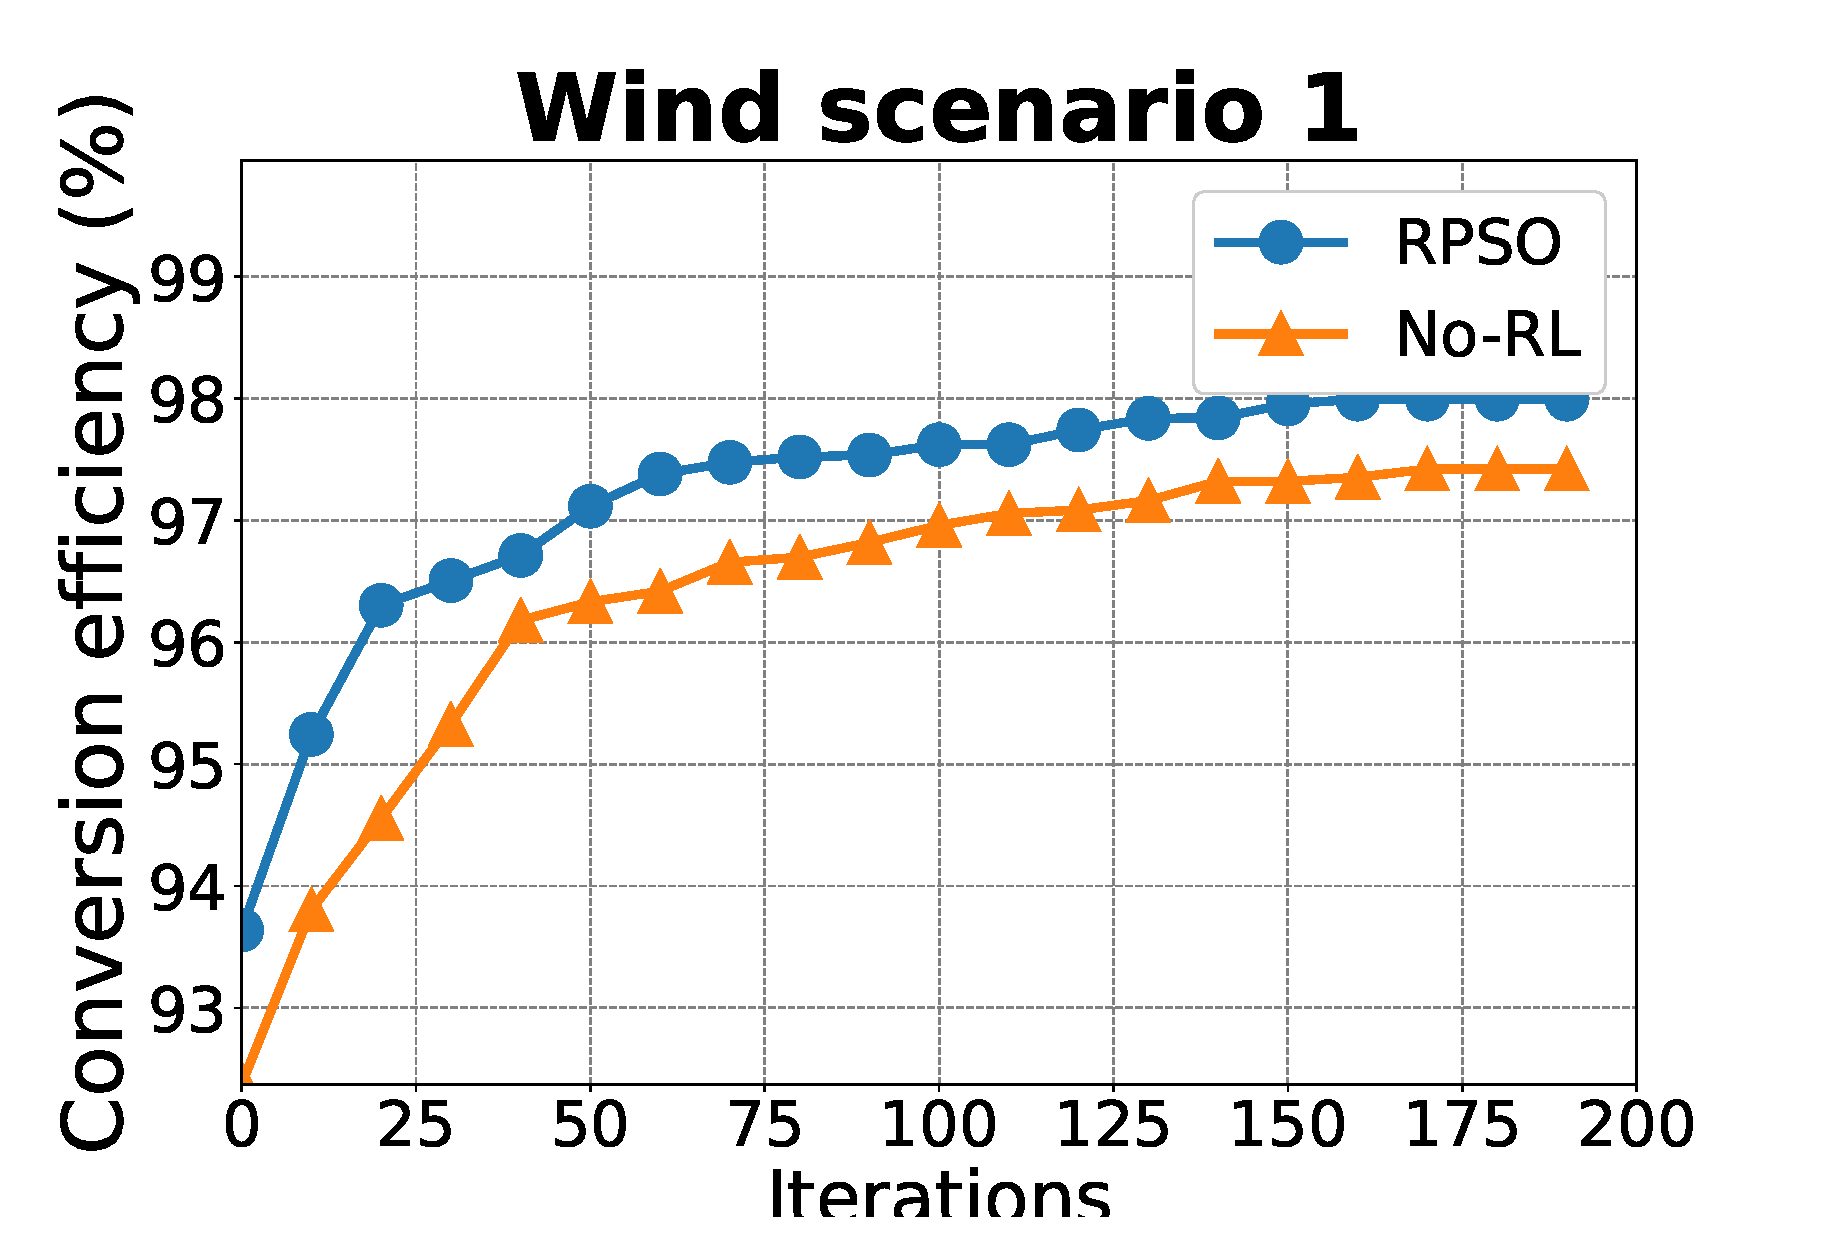
\includegraphics[width=\textwidth]{eta_S1.eps}
		\label{fig:sub1}
	\end{subfigure}
	% 第一行第二张图
	\begin{subfigure}{0.45\textwidth}
		\centering
		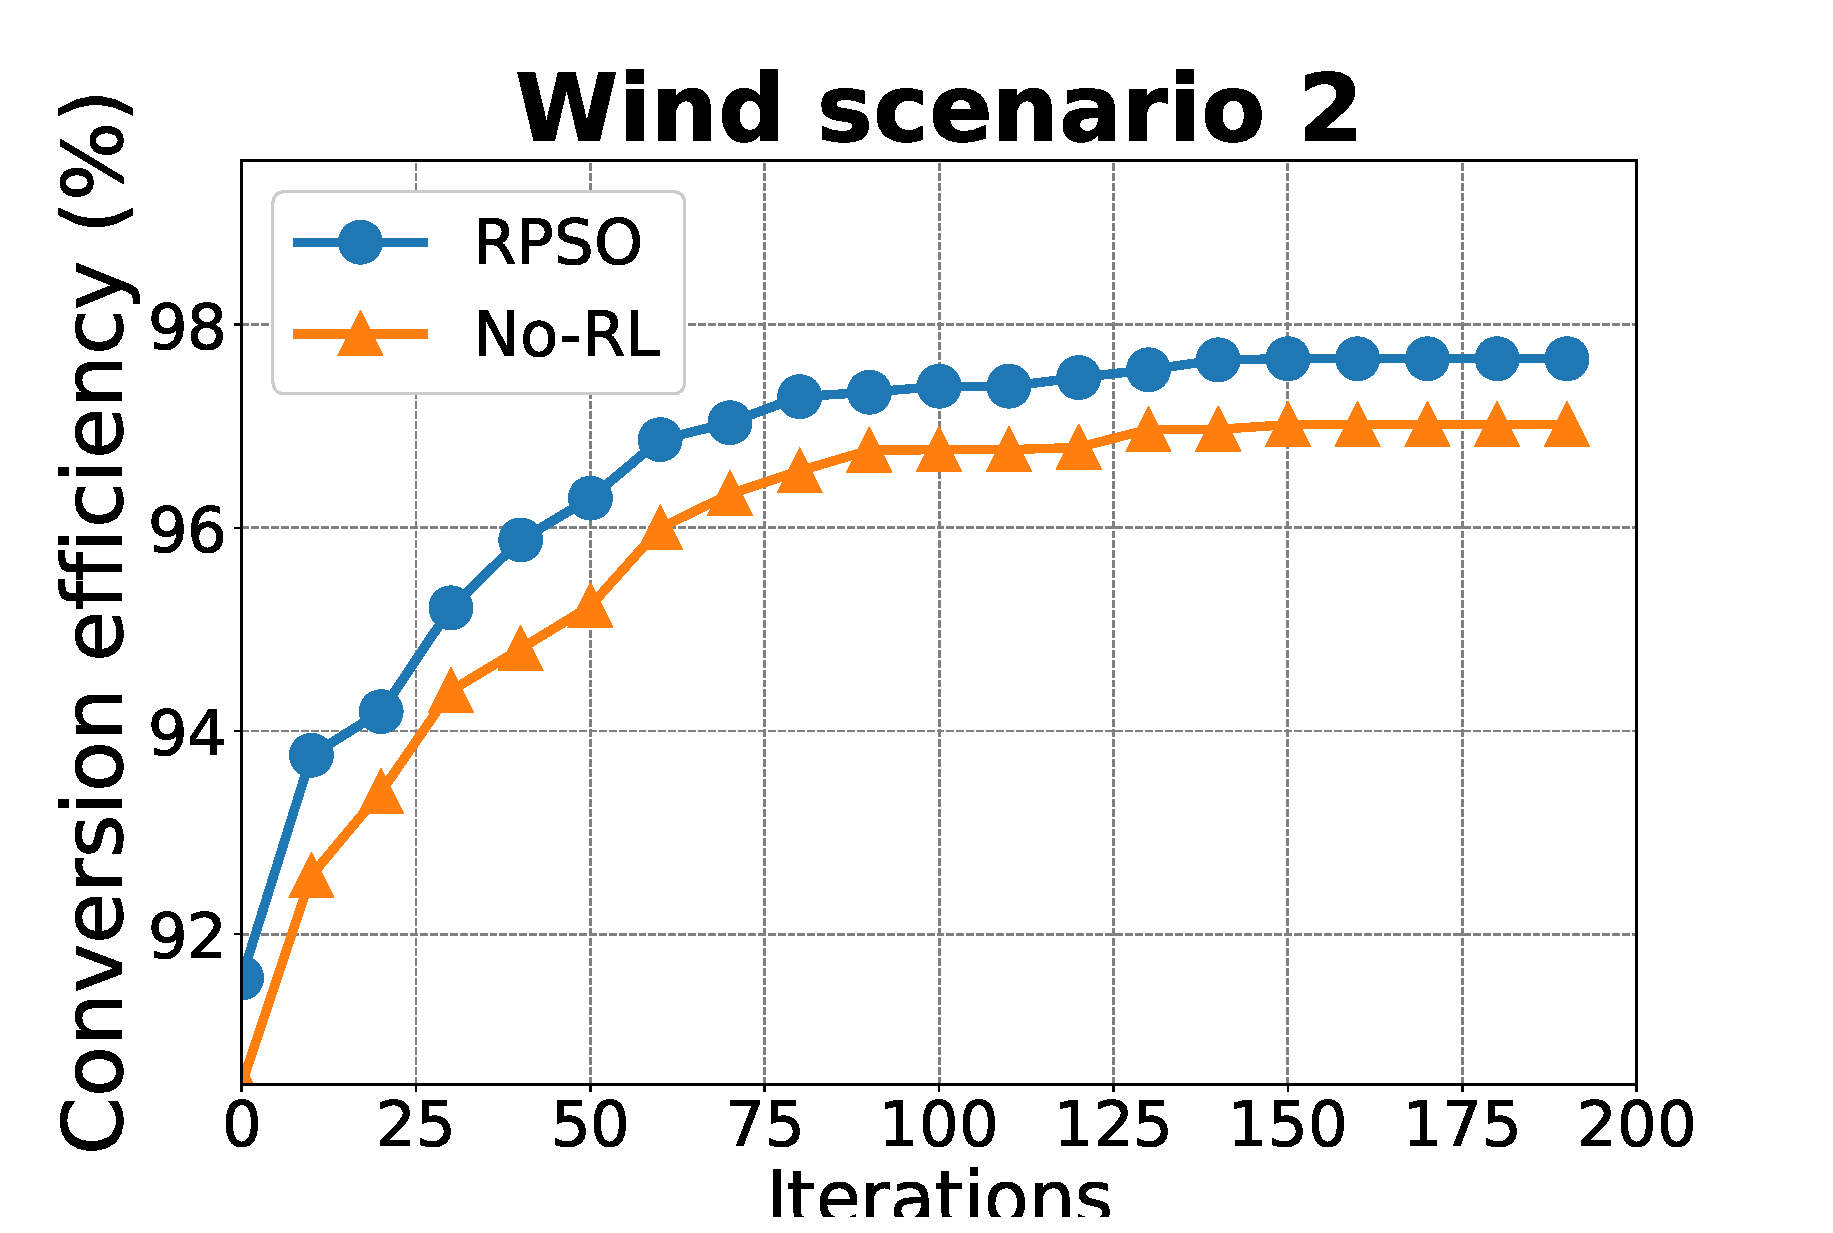
\includegraphics[width=\textwidth]{eta_S2.eps}
		\label{fig:sub2}
	\end{subfigure}
	% 换行
	%\vspace{0.5cm}
	
	% 第二行第一张图
	\begin{subfigure}{0.45\textwidth}
		\centering
		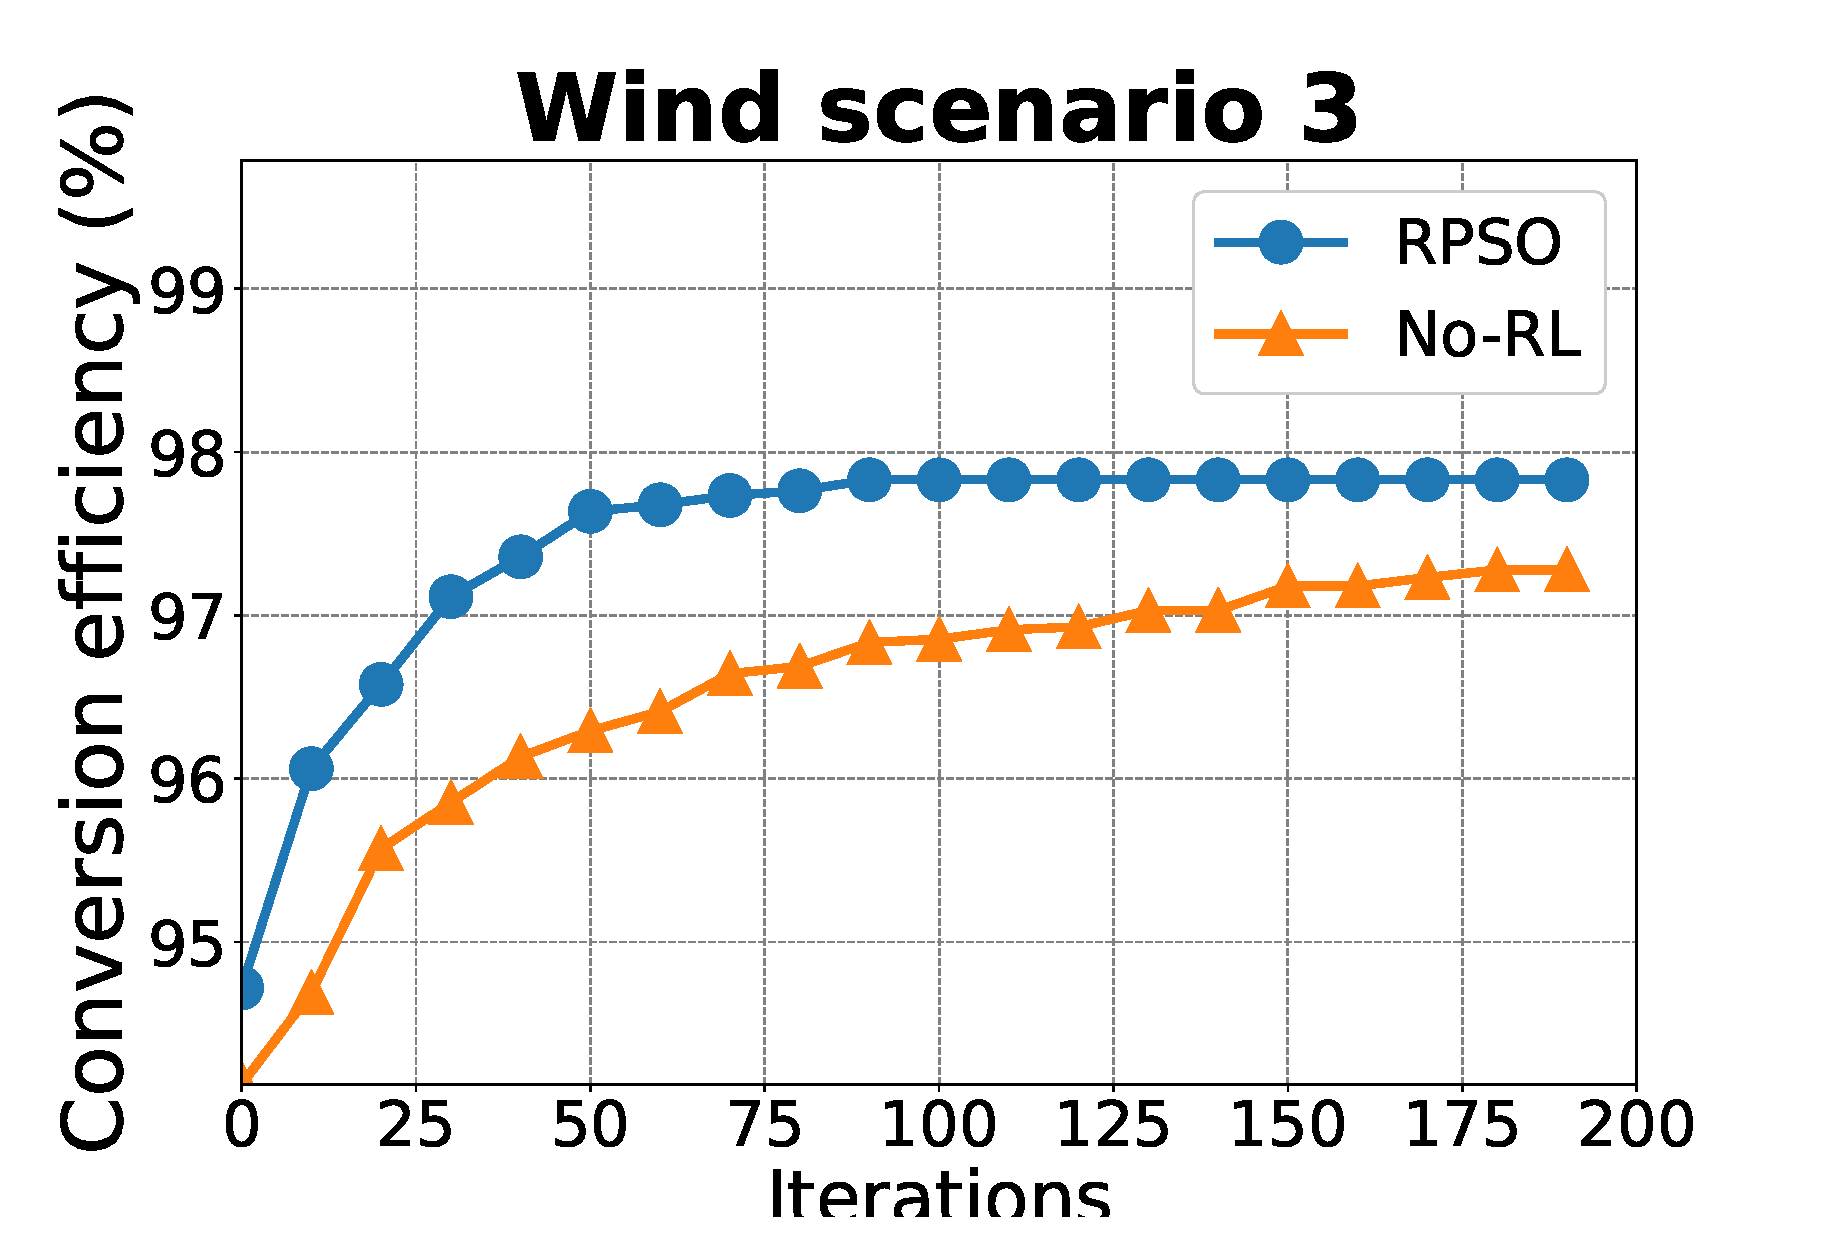
\includegraphics[width=\textwidth]{eta_S3.eps}
		\label{fig:sub3}
	\end{subfigure}
	% 第二行第二张图
	\begin{subfigure}{0.45\textwidth}
		\centering
		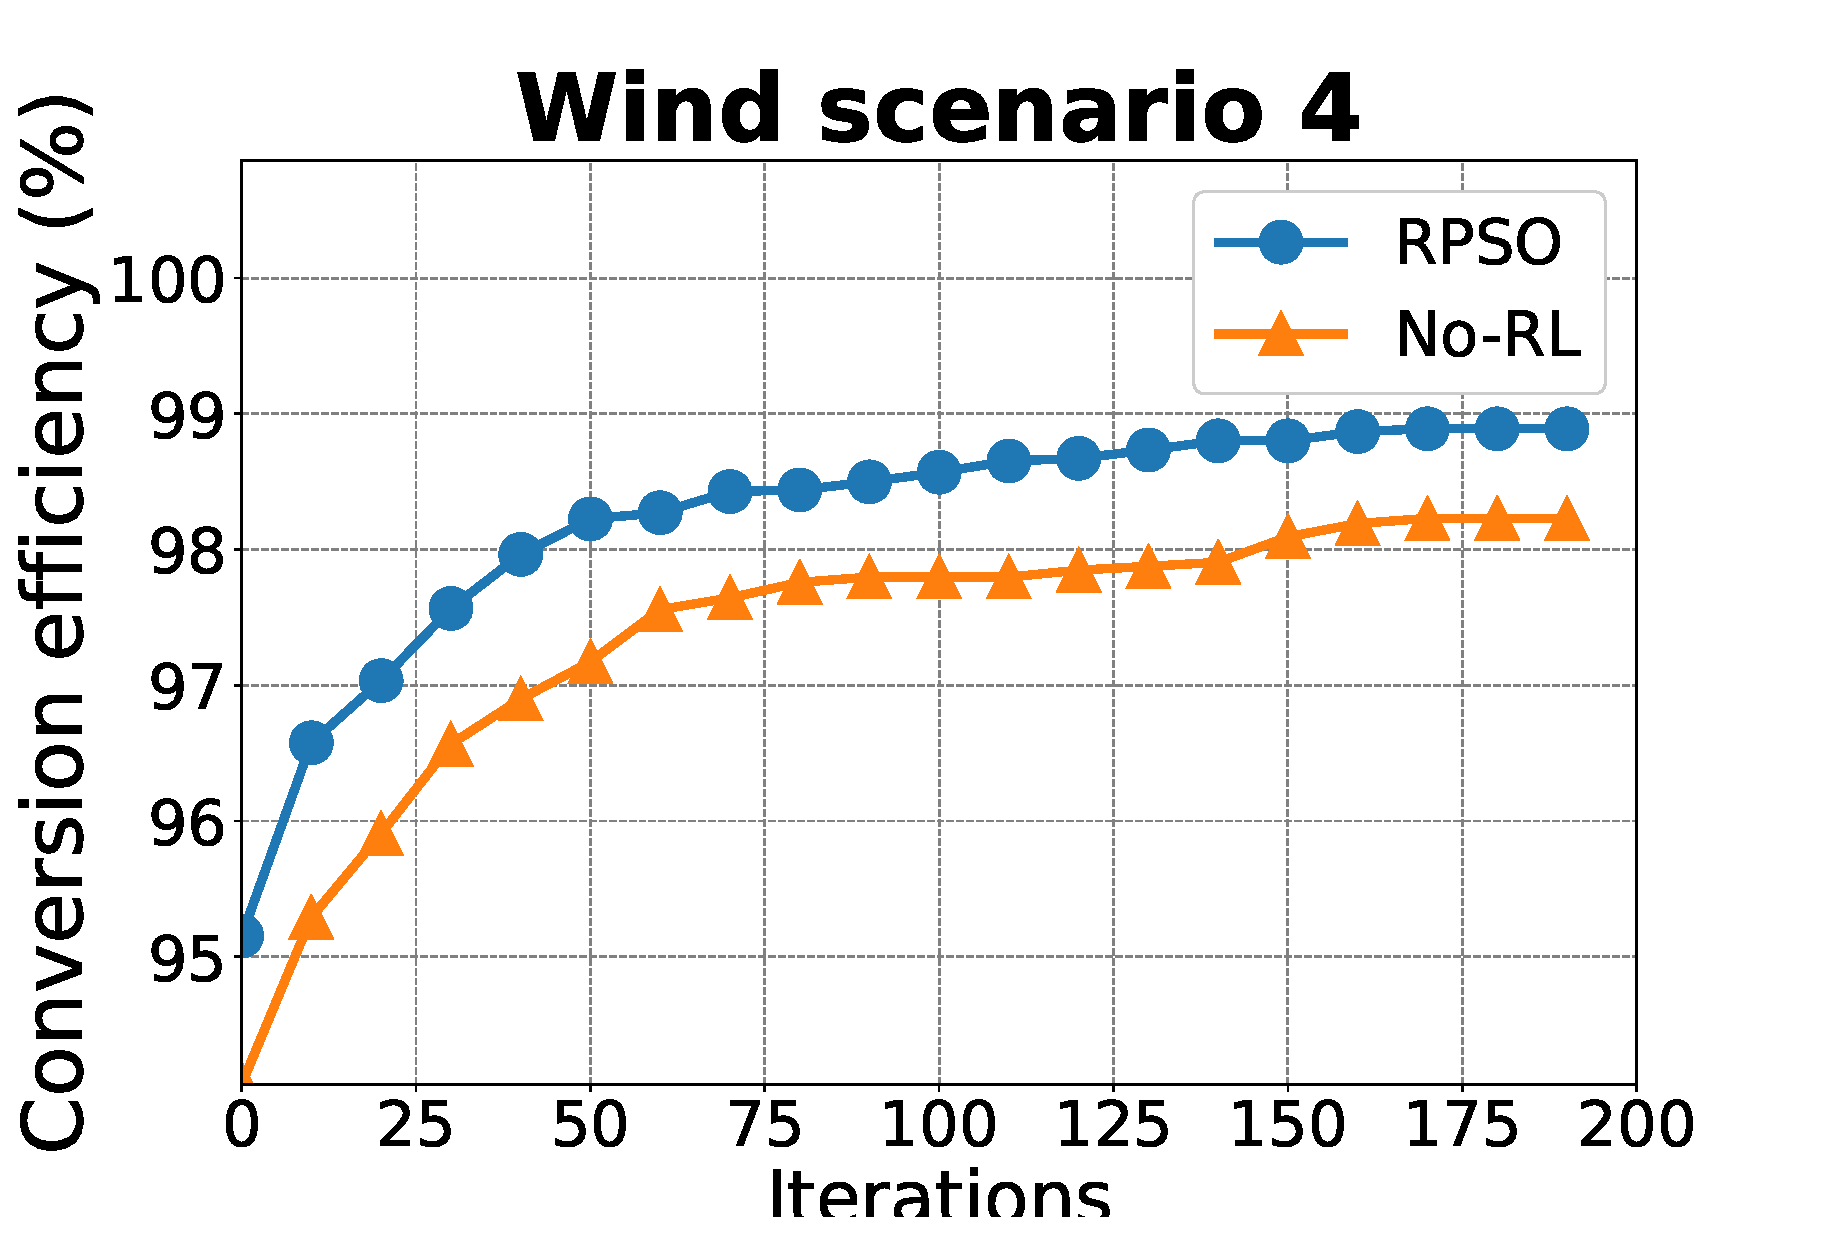
\includegraphics[width=\textwidth]{eta_S4.eps}
		\label{fig:sub4}
	\end{subfigure}
	
	\caption{\textcolor{blue}{Convergence comparison for four wind conditions with and without RL strategies.}}
	\label{fig:four_images}
\end{figure}
\begin{table}[t]
	\captionsetup{labelfont={color=black},font={color=black}}
	\centering
	\caption{Comparison of algorithm without RL strategy with RPSO output on four wind scenarios.}
	\label{norl}
	\linespread{1.1}
	\selectfont
	\resizebox{0.7\columnwidth}{!}{
	\begin{tabular}{ccccc}
		\hline
		&Methods& TN30 & TN35 & TN40 \\\hline
		\multirow{2}{*}{S 1}&RPSO   & \textbf{98.17 (±0.18)} &\textbf{97.21 (±0.44)}&\textbf{95.83 (±0.31)}  \\ \cline{2-5}
		&No-RL   & 97.62 (±0.29) &  96.42 (±0.28) & 95.38 (±0.00) \\ \hline
		
		\multirow{2}{*}{S 2}&RPSO  & \textbf{97.77 (±0.30)}& \textbf{96.71 (±0.34)}&\textbf{95.06 (±0.31)}  \\ \cline{2-5}
		&No-RL & 97.06 (±0.29)  & 95.77 (±0.25) & 94.18 (±0.25) \\ \hline
		
		\multirow{2}{*}{S 3}&RPSO  & \textbf{97.82 (±0.06)}& \textbf{97.07 (±0.21)}& \textbf{95.90 (±0.31)}  \\ \cline{2-5}
		&No-RL  & 97.51 (±0.11) & 96.61 (±0.21) & 95.70 (±0.20) \\ \hline
		
		\multirow{2}{*}{S 4}&RPSO  & \textbf{98.68 (±0.14)}& \textbf{98.14 (±0.17)}&\textbf{97.33 (±0.41)} \\ \cline{2-5}
		&No-RL  & 98.29 (±0.15) & 97.57 (±0.15) & 96.92 (±0.25)   \\ \hline		
		
	\end{tabular}}
\end{table}

\begin{table}[t]
	\captionsetup{labelfont={color=black},font={color=black}}
	\centering
	\caption{Statistical test of $p$-value with No-RL.}
	\label{hlcom}
	\linespread{1.1}
	\selectfont
	\resizebox{0.7\columnwidth}{!}{
	\begin{tabular}{cccccc}
		\hline
		&$-$&S1& S2 & S3 & S4 \\\hline
		&$ p $-value&1.95e-03   & 9.77e-04 &  9.77e-04  & 1.95e-03\\ \hline
	\end{tabular}
}
\end{table}
\section{Conclusion}\label{conclusion}
\textcolor{blue}{In this study, we propose an RPSO algorithm that integrates a PPO deep reinforcement learning strategy with the aim of accelerating the convergence of the PSO algorithm by combining historical information from the PPO and PSO strategies, as well as the ability to search for the global optimum, minimize the wake impact on the downstream turbines and maximize the energy output. Experimental evaluations are carried out in four different wind farm environments, considering turbine sizes of 30, 35 and 40, and comparisons with 12 SOTA algorithms for solving the WFLO problem show that our proposed RPSO is highly competitive. The experimental results demonstrate the convergence and robustness of our algorithm, and the ablation experiments highlight the key role of RL, which guides the global best particles and the historical best particles with appropriate weights in the subsequent iterations. RPSO can significantly enhance the power generation efficiency of wind farms by mitigating wake effects and reducing deployment costs in real-world scenarios, thereby promoting the sustainable and effective use of renewable energy.}

\section*{Acknowledgment}
This research was partially supported by the Japan Society for the Promotion of Science (JSPS) KAKENHI under Grant JP23K24899, and Japan Science and Technology Agency (JST) Support for Pioneering Research Initiated by the Next Generation (SPRING) under Grant JPMJSP2145.

\bibliographystyle{elsarticle-num-names}
\bibliography{reference_clean}

\end{document}

